%%%%%%%%%%%%%%%%%%%%%%%%%%%%%%%%%%%%%%%%%%%%%%%%%%%%%%%%%%%%%%%%%%%%%%%%%
%  Zawartość: Główny plik szablonu pracy dyplomowej (magisterskiej/inżynierskiej).
%  Opracował: Tomasz Kubik <tomasz.kubik@pwr.edu.pl>
%  Data: kwiecień 2016
%  Wersja: 0.2
%%%%%%%%%%%%%%%%%%%%%%%%%%%%%%%%%%%%%%%%%%%%%%%%%%%%%%%%%%%%%%%%%%%%%%%%%

\documentclass[a4paper,onecolumn,oneside,12pt,extrafontsizes]{memoir}
% W celu przygotowania wydruku do archiwum należy przesłonić komendę powyższą
% dwoma poniższymi komendami:
%\documentclass[a4paper,onecolumn,twoside,10pt]{memoir} 
%\renewcommand{\normalsize}{\fontsize{8pt}{10pt}\selectfont}

%\usepackage[cp1250]{inputenc} % jeśli kodowanie edytowanych plików to cp1250 
%\usepackage[utf8]{inputenc} % jeśli kodowanie edytowanych plików to UTF8
\usepackage[T1]{fontenc}
\usepackage[polish]{babel}
%\DisemulatePackage{setspace}
\usepackage{setspace}
\usepackage{tabularx}
\usepackage{color,calc}
%\usepackage{soul} % pakiet z komendami do podkreślania tekstu

\usepackage{ebgaramond} % pakiet z czcionkami garamond, potrzebny tylko do strony tytułowej, musi wystąpić przed pakietem tgtermes

%% Aby uzyskać polskie literki w pdfie (a nie zlepki) korzystamy z pakietu czcionek tgterms. 
%% W pakiecie tym są zdefiniowane klony czcionek Times o kształtach: normalny, pogrubiony, italic, italic pogrubiony.
%% W pakiecie tym brakuje czcionki o kształcie: slanted (podobny do italic). 
%% Jeśli w dokumencie gdzieś zostanie zastosowana czcionka slanted (np. po użyciu komendy \textsl{}), to
%% latex dokona podstawienia na czcionkę standardową i zgłosi to w ostrzeżeniu (warningu).
%% Ponadto tgtermes to czcionka do tekstu. Wszelkie matematyczne wzory będą sformatowane domyślną czcionką do wzorów.
%% Jeśli wzory mają być sformatowane z wykorzystaniem innych czcionek, trzeba to jawnie zadeklarować.

%% Po zainstalowaniu pakietu tgtermes może będzie trzeba zauktualizować informacje 
%% o dostępnych fontach oraz mapy. Można to zrobić z konsoli (jako administrator)
%% initexmf --admin --update-fndb
%% initexmf --admin --mkmaps

\usepackage{tgtermes}   
\renewcommand*\ttdefault{txtt}

% We wcześniejszej wersji szablonu korzystano z innych czcionek. Dla celów historycznych pozostawiono je w komentarzu
%\usepackage{mathptmx} % pakiet będący następcą pakietów times and mathptm, niestety polskie literki są zlepkami
%\usepackage{newtxtext,newtxmath} % pakiety dostarczające Times dla tekstów i wzorów matematycznych,  
%                                  rozwiązuje problemy występujące w mathptmx, ale wymaga zainstalowania
%                                  dodatkowych pakietów oraz uruchomienia updmap (konsola administratora)
%                                  niestety polskie literki są zlepkami
%\usepackage{newtxmath,tgtermes} % można też połączyć czcionki do tekstu i czcionki do wzorów

\usepackage{listings} % pakiet do prezentacji kodu. 
%Wcześniej był problem z polskimi znakami w otoczeniu lstlisting, stąd pozostawiono w komentarzu zastosowane wtedy rozwiązanie: 
\lstset{literate=%-
{ą}{{\k{a}}}1 {ć}{{\'c}}1 {ę}{{\k{e}}}1 {ł}{{\l{}}}1 {ń}{{\'n}}1 {ó}{{\'o}}1 {ś}{{\'s}}1 {ż}{{\.z}}1 {ź}{{\'z}}1 {Ą}{{\k{A}}}1 {Ć}{{\'C}}1 {Ę}{{\k{E}}}1 {Ł}{{\L{}}}1 {Ń}{{\'N}}1 {Ó}{{\'O}}1 {Ś}{{\'S}}1 {Ż}{{\.Z}}1 {Ź}{{\'Z}}1 }%{\ \ }{{\ }}1}

% Choć możliwe jest zastosowanie różnych pakietów formatujących tabele, zaleca się tego nie robić.
%\usepackage{longtable}
%\usepackage{ltxtable}
%\usepackage{tabulary}

%%%%%%%%%%%%%%%%%%%%%%%%%%%%%%%%%%%%%%%%%%%%%%%%%%%
%% Ustawienia odpowiedzialne za sposób łamania dokumentu
%% i ułożenie elementów pływających
%%%%%%%%%%%%%%%%%%%%%%%%%%%%%%%%%%%%%%%%%%%%%%%%%%%
%\hyphenpenalty=10000		% nie dziel wyrazów zbyt często
\clubpenalty=10000      %kara za sierotki
\widowpenalty=10000  % nie pozostawiaj wdów
\brokenpenalty=10000		% nie dziel wyrazów między stronami
\exhyphenpenalty=999999		% nie dziel słów z myślnikiem
\righthyphenmin=3			% dziel minimum 3 litery

%\tolerance=4500
%\pretolerance=250
%\hfuzz=1.5pt
%\hbadness=1450

\renewcommand{\topfraction}{0.95}
\renewcommand{\bottomfraction}{0.95}
\renewcommand{\textfraction}{0.05}
\renewcommand{\floatpagefraction}{0.35}

%%%%%%%%%%%%%%%%%%%%%%%%%%%%%%%%%%%%%%%%%%%%%%%%%%%
%%  Ustawienia rozmiarów: tekstu, nagłówka i stopki, marginesów
%%  dla dokumentów klasy memoir 
%%%%%%%%%%%%%%%%%%%%%%%%%%%%%%%%%%%%%%%%%%%%%%%%%%%
\setlength{\headsep}{10pt} 
\setlength{\headheight}{13.6pt} % wartość baselineskip dla czcionki 11pt tj. \small wynosi 13.6pt
\setlength{\footskip}{\headsep+\headheight}
\setlength{\uppermargin}{\headheight+\headsep+1cm}
\setlength{\textheight}{\paperheight-\uppermargin-\footskip-1.5cm}
\setlength{\textwidth}{\paperwidth-5cm}
\setlength{\spinemargin}{2.5cm}
\setlength{\foremargin}{2.5cm}
\setlength{\marginparsep}{2mm}
\setlength{\marginparwidth}{2.3mm}
%\settrimmedsize{297mm}{210mm}{*}
%\settrims{0mm}{0mm}	
\checkandfixthelayout[fixed] % konieczne, aby się dobrze wszystko poustawiało
%%%%%%%%%%%%%%%%%%%%%%%%%%%%%%%%%%%%%%%%%%%%%%%%
%%  Ustawienia odległości linii, wcięć, odstępów
%%%%%%%%%%%%%%%%%%%%%%%%%%%%%%%%%%%%%%%%%%%%%%%%
\linespread{1}
%\linespread{1.241}
\setlength{\parindent}{14.5pt}
%\setbeforesecskip{10pt plus 0.5ex}%{-3.5ex \@plus -1ex \@minus -.2ex}
%\setaftersecskip{10pt plus 0.5ex}%\onelineskip}
%\setbeforesubsecskip{8pt plus 0.5ex}%{-3.5ex \@plus -1ex \@minus -.2ex}
%\setaftersubsecskip{8pt plus 0.5ex}%\onelineskip}
%\setlength\floatsep{6pt plus 2pt minus 2pt} 
%\setlength\intextsep{12pt plus 2pt minus 2pt} 
%\setlength\textfloatsep{12pt plus 2pt minus 2pt} 

%%%%%%%%%%%%%%%%%%%%%%%%%%%%%%%%%%%%%%%%%%%%%%%%%%%
%%  Pakiety i komendy zastosowane tylko do zamieszczenia informacji o użytych komendach i fontach
%%  Normalnie nie są potrzebne, można je zamarkować podczas redakcji pracy
%%%%%%%%%%%%%%%%%%%%%%%%%%%%%%%%%%%%%%%%%%%%%%%%%%%
\usepackage{memlays}     % extra layout diagrams, zastosowane w szblonie do 'debuggowania', używa pakietu layouts
%\usepackage{layouts}
\usepackage{printlen} % pakiet do wyświetlania wartości zdefiniowanych długości, stosowany do 'debuggowania'
\uselengthunit{pt}
\makeatletter
\newcommand{\showFontSize}{\f@size pt} % makro wypisujące wielkość bieżącej czcionki
\makeatother
% do pokazania ramek można byłoby użyć:
%\usepackage{showframe} 


%%%%%%%%%%%%%%%%%%%%%%%%%%%%%%%%%%%%%%%%%%%%%%%%%%%
%%  Formatowanie list wyliczeniowych, wypunktowań i własnych otoczeń
%%%%%%%%%%%%%%%%%%%%%%%%%%%%%%%%%%%%%%%%%%%%%%%%%%%

% Domyślnie wypunktowania mają zadeklatorowane znaki, które nie występują w tgtermes
% Aby latex nie podstawiał w ich miejsca znaków z czcionki standardowej można zrobić podstawienie:
%    \DeclareTextCommandDefault{\textbullet}{\ensuremath{\bullet}}
%    \DeclareTextCommandDefault{\textasteriskcentered}{\ensuremath{\ast}}
%    \DeclareTextCommandDefault{\textperiodcentered}{\ensuremath{\cdot}}
% Jednak jeszcze lepszym pomysłem jest zdefiniowanie otoczeń z wykorzystaniem enumitem
\usepackage{enumitem} % pakiet pozwalający zarządzać formatowaniem list wyliczeniowych
\setlist{noitemsep,topsep=4pt,parsep=0pt,partopsep=4pt,leftmargin=*} % zadeklarowane parametry pozwalają uzyskać 'zwartą' postać wypunktowania bądź wyliczenia
\setenumerate{labelindent=0pt,itemindent=0pt,leftmargin=!,label=\arabic*.} % można zmienić \arabic na \alph, jeśli wyliczenia mają być z literkami
\setlistdepth{4} % definiujemy głębokość zagnieżdżenia list wyliczeniowych do 4 poziomów
\setlist[itemize,1]{label=$\bullet$}  % definiujemy, jaki symbol ma być użyty w wyliczeniu na danym poziomie
\setlist[itemize,2]{label=\normalfont\bfseries\textendash}
\setlist[itemize,3]{label=$\ast$}
\setlist[itemize,4]{label=$\cdot$}
\renewlist{itemize}{itemize}{4}

%%%http://tex.stackexchange.com/questions/29322/how-to-make-enumerate-items-align-at-left-margin
%\renewenvironment{enumerate}
%{
%\begin{list}{\arabic{enumi}.}
%{
%\usecounter{enumi}
%%\setlength{\itemindent}{0pt}
%%\setlength{\leftmargin}{1.8em}%{2zw} % 
%%\setlength{\rightmargin}{0zw} %
%%\setlength{\labelsep}{1zw} %
%%\setlength{\labelwidth}{3zw} % 
%\setlength{\topsep}{6pt}%
%\setlength{\partopsep}{0pt}%
%\setlength{\parskip}{0pt}%
%\setlength{\parsep}{0em} % 
%\setlength{\itemsep}{0em} % 
%%\setlength{\listparindent}{1zw} % 
%}
%}{
%\end{list}
%}

\makeatletter
\renewenvironment{quote}{
	\begin{list}{}
	{
	\setlength{\leftmargin}{1em}
	\setlength{\topsep}{0pt}%
	\setlength{\partopsep}{0pt}%
	\setlength{\parskip}{0pt}%
	\setlength{\parsep}{0pt}%
	\setlength{\itemsep}{0pt}
	}
	}{
	\end{list}}
\makeatother

%%%%%%%%%%%%%%%%%%%%%%%%%%%%%%%%%%%%%%%%%
%%  Pakiet do generowania indeksu (ważne, aby wstawić przed hyperref)
%%%%%%%%%%%%%%%%%%%%%%%%%%%%%%%%%%%%%%%%%
\DisemulatePackage{imakeidx}
\usepackage[makeindex,noautomatic]{imakeidx} % tutaj mówimy, żeby indeks nie generował się automatycznie, 

%\usepackage[noautomatic]{imakeidx} 
\makeindex

\makeatletter
%%%\renewenvironment{theindex}
							 %%%{\vskip 10pt\@makeschapterhead{\indexname}\vskip -3pt%
								%%%\@mkboth{\MakeUppercase\indexname}%
												%%%{\MakeUppercase\indexname}%
								%%%\vspace{-3.2mm}\parindent\z@%
								%%%\renewcommand\subitem{\par\hangindent 16\p@ \hspace*{0\p@}}%%
								%%%\phantomsection%
								%%%\begin{multicols}{2}
								%%%%\thispagestyle{plain}
								%%%\parindent\z@                
								%%%%\parskip\z@ \@plus .3\p@\relax
								%%%\let\item\@idxitem}
							 %%%{\end{multicols}\clearpage}
%%%
\makeatother


\usepackage{ifpdf}
%\newif\ifpdf \ifx\pdfoutput\undefined
%\pdffalse % we are not running PDFLaTeX
%\else
%\pdfoutput=1 % we are running PDFLaTeX
%\pdftrue \fi
\ifpdf
 \usepackage[pdftex,bookmarks,breaklinks,unicode]{hyperref}
 \usepackage[pdftex]{graphicx}
 \DeclareGraphicsExtensions{.pdf,.jpg,.mps,.png}
\pdfcompresslevel=9
\pdfoutput=1
\makeatletter
\AtBeginDocument{
  \hypersetup{
	pdfinfo={
    Title = {\@title},
    Author = {\@author},
    Subject={},
    Keywords={słowa kluczowe},
  }}
}
\makeatother
\else
\usepackage{graphicx}
\DeclareGraphicsExtensions{.eps,.ps,.jpg,.mps,.png}
\fi
\sloppy


%\graphicspath{{rys01/}{rys02/}}


%%%%%%%%%%%%%%%%%%%%%%%%%%%%%%%%%%%%%%%%%
% Metadane dla pdfa


%\ifpdf
%\pdfinfo{
   %/Author (Nicola Talbot)
   %/Title  (Creating a PDF document using PDFLaTeX)
   %/CreationDate (D:20040502195600)
   %/ModDate (D:\pdfdate)
   %/Subject (PDFLaTeX)
   %/Keywords (PDF;LaTeX)
%}
%\fi

% Deklaracja głębokościu numeracji
\setcounter{secnumdepth}{2}
\setcounter{tocdepth}{2}
\setsecnumdepth{subsection} % activating subsubsec numbering in doc


% Kropki po numerach sekcji
\makeatletter
\def\@seccntformat#1{\csname the#1\endcsname.\quad}
\def\numberline#1{\hb@xt@\@tempdima{#1\if&#1&\else.\fi\hfil}}
\makeatother

\renewcommand{\chapternumberline}[1]{#1.\quad}
\renewcommand{\cftchapterdotsep}{\cftdotsep}

%\definecolor{niceblue}{rgb}{.168,.234,.671}

% Czcionka do podpisów tabel i rysunków
\captionnamefont{\small}
\captiontitlefont{\small}
% makro pozwalające zmienić sposób wypisywania rozdziału
%\def\printchaptertitle##1{\fonttitle \space \thechapter.\space ##1} 

%\usepackage{ltcaption}
% The ltcaption package supports \CaptionLabelFont & \CaptionTextFont introduced by the NTG document classes
%\renewcommand\CaptionLabelFont{\small}
%\renewcommand\CaptionTextFont{\small}

% Przedefiniowanie etykiet w podpisach tabel i rysunków
%\AtBeginDocument{% 
        \addto\captionspolish{% 
        \renewcommand{\tablename}{Tab.}% 
}%} 

%\AtBeginDocument{% 
%        \addto\captionspolish{% 
%        \renewcommand{\chaptername}{Rozdział}% 
%}} 

%\AtBeginDocument{% 
        \addto\captionspolish{% 
        \renewcommand{\figurename}{Rys.}% 
}%}


%\AtBeginDocument{% 
        \addto\captionspolish{% 
        \renewcommand{\bibname}{Literatura}% 
}%}

%\AtBeginDocument{% 
        \addto\captionspolish{% 
        \renewcommand{\listfigurename}{Spis rysunków}% 
}%}

%\AtBeginDocument{% 
        \addto\captionspolish{% 
        \renewcommand{\listtablename}{Spis tabel}% 
}%}

%\AtBeginDocument{% 
        \addto\captionspolish

%%%%%%%%%%%%%%%%%%%%%%%%%%%%%%%%%%%%%%%%%%%%%%%%%%%%%%%%%%%%%%%%%%                  
%% Definicje stopek i nagłówków
%%%%%%%%%%%%%%%%%%%%%%%%%%%%%%%%%%%%%%%%%%%%%%%%%%%%%%%%%%%%%%%%%%                  
\addtopsmarks{headings}{%
\nouppercaseheads % added at the beginning
}{%
\createmark{chapter}{both}{shownumber}{}{. \space}
%\createmark{chapter}{left}{shownumber}{}{. \space}
\createmark{section}{right}{shownumber}{}{. \space}
}%use the new settings

\makeatletter
\copypagestyle{outer}{headings}
\makeoddhead{outer}{}{}{\small\itshape\rightmark}
\makeevenhead{outer}{\small\itshape\leftmark}{}{}
\makeoddfoot{outer}{\small\@author:~\@titleShort}{}{\small\thepage}
\makeevenfoot{outer}{\small\thepage}{}{\small\@author:~\@title}
\makeheadrule{outer}{\linewidth}{\normalrulethickness}
\makefootrule{outer}{\linewidth}{\normalrulethickness}{2pt}
\makeatother

% fix plain
\copypagestyle{plain}{headings} % overwrite plain with outer
\makeoddhead{plain}{}{}{} % remove right header
\makeevenhead{plain}{}{}{} % remove left header
\makeevenfoot{plain}{}{}{}
\makeoddfoot{plain}{}{}{}

\copypagestyle{empty}{headings} % overwrite plain with outer
\makeoddhead{empty}{}{}{} % remove right header
\makeevenhead{empty}{}{}{} % remove left header
\makeevenfoot{empty}{}{}{}
\makeoddfoot{empty}{}{}{}


%%%%%%%%%%%%%%%%%%%%%%%%%%%%%%%%%%%%%%%
%% Definicja strony tytułowej 
%%%%%%%%%%%%%%%%%%%%%%%%%%%%%%%%%%%%%%%
\makeatletter
%Uczelnia
\newcommand\uczelnia[1]{\renewcommand\@uczelnia{#1}}
\newcommand\@uczelnia{}
%Wydział
\newcommand\wydzial[1]{\renewcommand\@wydzial{#1}}
\newcommand\@wydzial{}
%Kierunek
\newcommand\kierunek[1]{\renewcommand\@kierunek{#1}}
\newcommand\@kierunek{}
%Specjalność
\newcommand\specjalnosc[1]{\renewcommand\@specjalnosc{#1}}
\newcommand\@specjalnosc{}
%Tytuł po angielsku
\newcommand\titleEN[1]{\renewcommand\@titleEN{#1}}
\newcommand\@titleEN{}
%Tytuł krótki
\newcommand\titleShort[1]{\renewcommand\@titleShort{#1}}
\newcommand\@titleShort{}
%Promotor
\newcommand\promotor[1]{\renewcommand\@promotor{#1}}
\newcommand\@promotor{}

%\usepackage[absolute]{textpos} % zamarkowano, bo ostatecznie wykorzystano otoczenie picture

\def\maketitle{%
  \pagestyle{empty}%
%%\garamond 
	\fontfamily{\ebgaramond@family}\selectfont % na stronie tytułowej czcionka garamond
%%%%%%%%%%%%%%%%%%%%%%%%%%%%%%%%%%%%%	
%% Poniżej, w otoczniu picture, wstawiono tytuł i autora. 
%% Tytuł (z autorem) musi znaleźć się w obszarze 
%% odpowiadającym okienku 110mmx75mm, którego lewy górny róg 
%% jest w położeniu 77mm od lewej i 111mm od górnej  krawędzi strony 
%% (tak wynika z wycięcia na okładce). 
%% Poniższy kod musi być użyty dokładnie w miejscu gdzie jest.
%% Jeśli tytuł nie mieści się w okienku, to należy tak pozmieniać 
%% parametry użytych komend, aby ten przydługi tytuł jednak 
%% upakować go do okienka.
%%
%% Sama okładka (kolorowa strona z wycięciem, do pobrania z dydaktyki) 
%% powinna być przycięta o 3mm od każdej z krawędzi.
%% Te 3mm pewnie zostawiono na ewentualne spady czy też specjalną oprawę.
%%%%%%%%%%%%%%%%%%%%%%%%%%%%%%%%%%%%%	
\newlength{\tmpfboxrule}
\setlength{\tmpfboxrule}{\fboxrule}
\setlength{\fboxsep}{2mm}
\setlength{\fboxrule}{0mm} 
%\setlength{\fboxrule}{0.1mm} %% jeśli chcemy zobaczyć ramkę
\setlength{\unitlength}{1mm}
\begin{picture}(0,0)
\put(26,-124){\fbox{
\parbox[c][71mm][c]{104mm}{\centering%\lineskip=34pt 
\fontsize{16pt}{18pt}\selectfont \@title\\[5mm]
\fontsize{16pt}{18pt}\selectfont \@titleEN\\[20mm]
\fontsize{16pt}{18pt}\selectfont AUTOR:\\[2mm]
\fontsize{14pt}{16pt}\selectfont \@author}
}
}
\end{picture}
\setlength{\fboxrule}{\tmpfboxrule} 
%%%%%%%%%%%%%%%%%%%%%%%%%%%%%%%%%%%%%
%% Reszta strony z nazwą uczelni, wydziału, kierunkiem, specjalnością
%% promotorem, oceną pracy, miastem i rokiem
	{\centering%\vspace{-1cm}
		{\fontsize{22pt}{24pt}\selectfont \@uczelnia}\\[0.4cm]
		{\fontsize{22pt}{24pt}\selectfont \@wydzial}\\[0.5cm]
		  \hrule %\vspace*{0.7cm}
	}
{\flushleft\fontsize{14pt}{16pt}\selectfont%
\begin{tabular}{ll}
KIERUNEK: & \@kierunek\\
SPECJALNOŚĆ: & \@specjalnosc\\
\end{tabular}\\[1.3cm]
}
{\centering
{\fontsize{32pt}{36pt}\selectfont PRACA DYPLOMOWA}\\[0.5cm]
{\fontsize{32pt}{36pt}\selectfont INŻYNIERSKA}\\[2.5cm]
}
\vfill
\begin{tabularx}{\linewidth}{p{6cm}l}
		&{\fontsize{16pt}{18pt}\selectfont PROWADZĄCY PRACĘ:}\\[2mm] %UWAGA: tutaj jest miejsce na nazwisko promotora pracy
		&{\fontsize{14pt}{16pt}\selectfont \@promotor}\\[10mm]
		&{\fontsize{16pt}{18pt}\selectfont OCENA PRACY:}\\[20mm]
	\end{tabularx}
\vspace{2cm}
\hrule\vspace*{0.3cm}
{\centering
{\fontsize{16pt}{18pt}\selectfont \@date}\\[0cm]
}
%\ungaramond
\normalfont
 \cleardoublepage
}
\makeatother
%%%%%%%%%%%%%%%%%%%%%%%%%%%%%%%%%%%%%%%%%

%\AtBeginDocument{\addtocontents{toc}{\protect\thispagestyle{empty}}}




%%%%%%%%%%%%%%%%%%%%%%%%%%%%%%%%%%%%%%%%%
%%  Metadane dokumentu 
%%%%%%%%%%%%%%%%%%%%%%%%%%%%%%%%%%%%%%%%%
\title{Platforma internetowa zrzeszająca zawodników uprawiających amatorsko sporty zespołowe}
\titleShort{Platforma internetowa zrzeszająca zawodników uprawiających amatorsko sporty...}
\titleEN{Web platform for players practicing amateur team sports}
\author{Bartosz Pogoda}
\uczelnia{POLITECHNIKA WROCŁAWSKA}
\wydzial{WYDZIAŁ ELEKTRONIKI}
\kierunek{INFORMATYKA}
\specjalnosc{INŻYNIERIA SYSTEMÓW INFORMATYCZNYCH}
\promotor{dr inż. Marek Piasecki, Jednostka????}
\date{WROCŁAW, 2018}

% Ustawienie odstępu od góry w nienumerowanych rozdziałach oraz wykazach:
% Spis treści, Spis tabel, Spis rysunków, Indeks rzeczowy

%\newlength{\linespace}
%\setlength{\linespace}{-\beforechapskip-\topskip+\headheight+\topsep}
%\makechapterstyle{noNumbered}{%
%\renewcommand\chapterheadstart{\vspace*{\linespace}}
%}

%% powyższa komenda załatwia to, co robią komendy poniższe dla spisów
%\renewcommand*{\tocheadstart}{\vspace*{\linespace}}
%\renewcommand*{\lotheadstart}{\vspace*{\linespace}}
%\renewcommand*{\lofheadstart}{\vspace*{\linespace}}

%%%%%%%%%%%%%%%%%%%%%%%%%%%%%%%%%%%%%%%%%
%                  Początek dokumentu 
%%%%%%%%%%%%%%%%%%%%%%%%%%%%%%%%%%%%%%%%%
%\includeonly{skroty,rozdzial01} % jeśli chcemy kompilować tylko fragmenty, to można tu je wpisać

\begin{document}
% Tutaj można przełączyć odstęp między liniami
%\SingleSpacing
%\OnehalfSpacing
%\DoubleSpacing

%\settypeoutlayoutunit{cm} % do debugowania
%\typeoutstandardlayout    % wypisuje na stdout informacje o ustawieniach
\maketitle

\newpage
\thispagestyle{empty}
\mbox{}\vfill
\noindent\begin{tabular}{@{}ll} Opracował: & Tomasz Kubik <tomasz.kubik@pwr.edu.pl>\\
 Data: & maj 2016 
 \end{tabular}\\[15mm]
\noindent
\includegraphics[width=3cm]{by-nc-sa}\newline
{\normalfont 
Szablon jest udostępniany na licencji Creative Commons: \emph{Uznanie autorstwa -- Użycie niekomercyjne -- Na tych samych warunkach, 3.0 Polska}, Wrocław 2016. \\[2pt]
Oznacza to, że wszystkie zawarte  nim treści można kopiować i  wykorzystywać do celów niekomercyjnych, a także tworzyć na ich podstawie utwory zależne pod warunkiem podania autora i~nazwy licencjodawcy oraz udzielania na utwory zależne takiej samej licencji. Tekst licencji jest dostępny pod adresem: \url{http://creativecommons.org/licenses/by-nc-sa/3.0/pl/}.}
\newpage


\chapterstyle{noNumbered}
\pagestyle{outer}
\mbox{}\pdfbookmark[0]{Spis treści}{spisTresci.1}
\tableofcontents* 

\newpage
\mbox{}\pdfbookmark[0]{Spis rysunków}{spisRysunkow.1}
%\addcontentsline{toc}{chapter}{Spis rysunków}
\listoffigures*
\begin{flushleft}

\end{flushleft}
%{%
%\let\oldnumberline\numberline%
%\renewcommand{\numberline}{\figurename~\oldnumberline}%
%\listoffigures%
%}


\newpage
\mbox{}\pdfbookmark[0]{Spis tabel}{spisTabel.1}
%\addcontentsline{toc}{chapter}{Spis tabel}
\listoftables*

\chapter*{Skróty}\mbox{}\pdfbookmark[0]{Skróty}{skroty.1}
\label{sec:skroty}
\noindent
\begin{description}
  \item [OGC] (ang.\ \emph{Open Geospatial Consortium}) %-- jednostka arytmetyczno--logiczna
  \item [XML] (ang.\ \emph{eXtensible Markup Language})
  \item [SOAP] (ang.\ \emph{Simple Object Access Protocol})
  \item [WSDL] (ang.\ \emph{Web Services Description Language})
  \item [UDDI] (ang.\ \emph{Universal Description Discovery and Integration})
  \item [GIS] (ang.\ \emph{Geographical Information System})
  \item [SDI] (ang.\ \emph{Spatial Data Infrastructure})
  \item [ISO] (ang.\ \emph{International Standards Organization})
  \item [WMS] (ang.\ \emph{Web Map Service})
  \item [WFS] (ang.\ \emph{Web Feature Service})
  \item [WPS] (ang.\ \emph{Web Processing Service})
  \item [GML] (ang.\ \emph{Geography Markup Language})
  \item [SRG] (ang.\ \emph{Seeded Region Growing})
  \item [SOA] (ang.\ \emph{Service Oriented Architecture })
  \item [IT] (ang.\ \emph{Information Technology })
\end{description}
 %skróty można sobie pominąć
\chapterstyle{default}
\chapter{Wstęp}
\section{Wprowadzenie}
Niniejszy dokument powstał z myślą o ujednoliceniu sposobu redagowania prac dyplomowych. Jego źródła mają pełnić rolę szablonu nowoedytowanej pracy, zaś treść powinna być interpretowana jako zestaw zaleceń i uwag o charakterze technicznym (dotyczących takich zagadnień, jak: formatowanie tekstu, załączanie rysunków, układ strony itp.) oraz stylistycznym (odnoszących się do stylu wypowiedzi, sposobów tworzenia referencji itp.).

Szablon przygotowano do kompilacji pdflatexem w konfiguracji: \texttt{MiKTeX} (windowsowa dystrybucja latexa) + \texttt{TeXnicCenter} (środowisko do edycji i kompilacji projektów latexowych) + \texttt{SumatraPDF} (przeglądarka pdfów z nawigacją zwrotną) + JabRef (opcjonalny edytor bazy danych bibliograficznych). Jest to zalecany zestaw narzędzi do edycji pracy w systemie Windows. Można je pobrać ze stron internetowych, których adresy zamieszczono w tabeli~\ref{tab:narzedzia}.
\begin{table}[htb] \small
\centering
\caption{Wykaz zalecanych narzędzi do kompilacji szablonu (adresy internetowe ważne na dzień 1.04.2016)}
\label{tab:narzedzia}
\begin{tabularx}{\linewidth}{|c|c|X|p{6cm}|} \hline\
Narzędzie & Wersja & Opis & Adres \\ \hline\hline
MiKTeX & 2.9 & Zalecana jest instalacja \texttt{Basic MiKTeX} z dystrubucji 32 lub 64 bitowej. Brakujące pakiety będą się doinstalowywać podczas kompilacji projektu. &
\url{http://miktex.org/download} \\ \hline
TexnicCenter & 2.02 &  Można pobrać 32 lub 64 bitową wersję & \url{http://www.texniccenter.org/download/} \\ \hline
SumatraPDF & 3.1.1 & Można pobrać 32 lub 64 bitową wersję & \url{http://www.sumatrapdfreader.org/download-free-pdf-viewer.html} \\ \hline
JabRef & 3.3 & Można pobrać 32 lub 64 bitową wersję & \url{http://www.fosshub.com/JabRef.html} \\ \hline
\end{tabularx}
\end{table}
Nic nie stoi jednak na przeszkodzie, aby szablon ten dostosować do wykorzystania z użyciem innych narzędzi. Dostosowanie to mogłoby polegać na zmianie kodowania plików i korekcie deklaracji kodowania znaków w dokumencie głównym (co opisano dalej).

W kodzie źródłowym szablonu zamieszczono komentarze z uwagami pozwalającymi lepiej zrozumieć znaczenie używanych komend. Komentarze te nie są widoczne w pliku \texttt{Dokument.pdf}, który powstaje jako wynik kompilacji szablonu. 


%%%2. środowisko do pisania kodu latexa: 
%%%( )
%%%3. viewer pdf-ów, pozwalający na nawigację zwrotną: Sumatra PDF 3.0
%%%(http://www.sumatrapdfreader.org/download-free-pdf-viewer.html)
%%%
%%%- o konfiguracji texniccenter do współdziałania z sumatra pdf można poczytać sobie na stronie:
%%%http://tex.stackexchange.com/questions/116981/how-to-configure-texniccenter-2-0-with-sumatra-2013-2014-2015-version
%%%(można znaleźć też inne tutoriale)
%%%
%%%4. środowisko do zarządzania bibliografią: JabRef
%%%(http://jabref.sourceforge.net/download.php)
%%%
%%%Polecam też instalację pod windowsami następujących narzędzi:
%%%- Sumatra PDF - przeglądarka pdf umożliwiająca nawigację pomiędzy
%%%edytowanym tekstem a przeglądanym dokumentem (podglądanie tekstu w
%%%TeXnicCenter umieszcza kursor w odpowiednim miejscu w pdfie, podwójne
%%%kliknięcie w pdfie ustawia kursor w edytorze tekstu).
%%%- JabRef - narzędzie do przygotowywania bibliografii.
%%%
%%%
%%%Uwaga: tytuł powinien zmieścić się w okienku kolorowej okładki (którą
%%%powinna dostarczyć uczelniana administracja). Proszę posterować
%%%parametrami, aby "wpasować" w okienko własny tekst.
%%%
%%%Do ASAPa należy wprowadzić pracę dyplomową/projekt inżynierski w pliku o nazwie:
%%%
%%%W04_[nr albumu]_[rok kalendarzowy]_[rodzaj pracy] (szczegółowa instrukcja pod adresem asap.pwr.edu.pl)
%%%
           %%%Przykładowo:
        %%%­W04_123456_2015_praca inżynierska.pdf     - praca dyplomowa inżynierska
        %%%W04_123456_2015_projekt inżynierski.pdf   - projekt inżynierski
        %%%W04_123456_2015_praca magisterska.pdf  - praca dyplomowa magisterska
%%%
              %%%rok kalendarzowy ? rok realizacji kursu „Praca dyplomowa” (nie rok obrony) 
\chapter{Praca z szablonem}
\section{Organizacja szablonu}
Szablon składa się z pliku głównego, plików z kodem kolejnych rozdziałów i dodatków (włączanych do kompilacji w dokumencie głównym), katalogów z plikami grafik (włączanymi do rysunków w rozdziałach), pliku ze skrótami (opcjonalny), pliku z danymi bibliograficznymi (plik \texttt{dokumentacja.bib}). Taki ,,układ'' zapewnia porządek oraz pozwala na selektywną kompilację rozdziałów. Wyjaśniając to dokładniej, podczas tworzenia szablonu przyjęto następującą konwencję:
\begin{itemize}
\item Plikiem głównym jest plik \texttt{Dyplom.tex}. To w nim znajdują się deklaracje wszystkich używanych styli, definicje makr oraz ustawień, jak również polecenie \verb+\begin{document}+.
\item Teksty rozdziałów są redagowane w osobnych plikach o nazwach zawierających numer rozdziału. Pliki te zamieszczone są w katalogu głównym (tym samym, co plik \texttt{Dyplom.tex}). I~tak \texttt{rozdzial01.tex} to plik pierwszego rozdziału (ze Wstępem), \texttt{rozdzial02.tex} to plik z treścią drugiego rozdziału itd. 
\item Teksty dodatków są redagowany w osobnych plikach o nazwach zawierających literę dodatku. Pliki te, podobnie do plików z tekstem rozdziałów, zamieszczane są w katalogu głównym. I~tak \texttt{dodatekA.tex} oraz \texttt{dodatekB.tex} to, odpowiednio, pliki z treścią dodatku A oraz dodatku B.
\item Pewnym wyjątkiem od reguły nazewniczej w przypadku plików z tekstem rozdziałów i dodatków jest plik \texttt{skroty.tex}. Jest to plik, w którym zamieszczono wykaz użytych skrótów. W jego nazwie nie występuje żaden numer czy porządkowa litera. 
\item Każdemu rozdziałowi i dodatkowi towarzyszy katalog przeznaczony do składowania dołączanych w nim grafik. I tak \texttt{rys01} to katalog na pliki z grafikami dołączanymi do rozdziału pierwszego, \texttt{rys02} to katalog na pliki z grafikami dołączanymi do rozdziału drugiego itd.
Podobnie \texttt{rysA} to katalog na pliki z grafikami dołączanymi w dodatku A itd.
\item W katalogu głównym zamieszczany jest plik \texttt{dokumentacja.bib} zawierający bazę danych bibliograficznych.
\end{itemize}

\begin{table}[htb]
\centering\small
\caption{Pliki źródłowe szablonu oraz wyniki kompilacji}
\label{tab:szablon}
\begin{tabularx}{\linewidth}{|p{.55\linewidth}|X|}\hline
Źródła & Wyniki kompilacji \\ \hline\hline
\verb?Dokument.tex? - dokument główny\newline
\verb?Dokument.tcp? -- szablon projektu \texttt{MiKTeX}\newline
\verb?rozdzial01.tex? -- plik rozdziału \texttt{01}\newline
\verb?...?\newline
\verb?dodatekA.tex? -- plik dodatku \texttt{A}\newline
\verb?...?\newline
\verb?rys01? -- katalog na rysunki do rozdziału \texttt{01}\newline
\verb?   |- fig01.png? -- plik grafiki\newline
\verb?   |- ...?\newline
\verb?...?\newline
\verb?rysA? -- katalog na rysunki do dodatku \texttt{A}\newline
\verb?   |- fig01.png? -- plik grafiki\newline
\verb?   |- ...?\newline
\verb?...?\newline
\verb?dokumentacja.bib? -- plik danych bibliograficznych\newline
\verb?Dyplom.ist? -- plik ze stylem indeksu\newline
\verb?by-nc-sa.png? -- plik z ikonami CC\newline
 &
\verb?Dyplom.bbl?\newline
\verb?Dyplom.blg?\newline
\verb?Dyplom.ind?\newline
\verb?Dyplom.idx?\newline
\verb?Dyplom.lof?\newline
\verb?Dyplom.log?\newline
\verb?Dyplom.lot?\newline
\verb?Dyplom.out?\newline
\verb?Dyplom.pdf? -- dokument wynikowy\newline
\verb?Dyplom.syntex?\newline
\verb?Dyplom.toc?\newline
\verb?Dyplom.tps?\newline
\verb?*.aux?\newline 
\verb?Dyplom.synctex?\newline\\
\hline
\end{tabularx}
\end{table}

Szablon przygotowano w systemie Windows stosując kodowanie \texttt{cp1250}. Można go wykorzystać również w innych systemach i przy innych kodowaniach. Jednakże wtedy konieczna jest korekta dokumentu \texttt{Dyplom.tex} odpowiednio do wybranego przypadku. Korekta ta polegać może na zamianie polecenia \verb+\usepackage[cp1250]{inputenc}+  na polecenie \verb+\usepackage[utf8]{inputenc}+ oraz konwersji kodowania istniejących plików ze źródłem latexowego kodu (plików o rozszerzeniu \texttt{*.tex} oraz \texttt{*.bib}).

Samo kodowanie plików może być źródłem paru problemów. Chodzi o to, że użytkownicy pracujący z edytorami tekstów pod linuxem mogą generować pliki zakodowane w UTF-8 bez BOM lub z BOM, a pod windowsem -- pliki z kodowaniem znaków \texttt{cp1250} zakodowanych w~ANSI. A z takimi plikami różne edytory różnie sobie radzą (w szczególności edytor TeXnicCenter czasami z niewiadomego powodu traktuje zawartość pliku jako UTF8 lub ANSI -- chyba sprawdza, czy w bufore nie ma jakichś znaków specjalnych i na tej podstawie interpretuje kodowanie). Bywa, że choć wszystko wygląda OK to jednak kompilacja latexowa ,,nie idzie''. Problemem mogą być właśnie pierwsze bajty, których nie widać w edytorze. 

Kodowanie znaków jest istotne również przy edytowaniu bazy danych bibliograficznych (pliku \texttt{dokumentacja.bib}). Aby \texttt{bibtex} poprawnie interpretował polskie znaki plik \texttt{dokumentacja.bib} powinien być zakodowany w ANSI, CR+LF (dla ustawień jak w szablonie). Do konwersji kodowania można użyć Notepad++ (jest tam opcja ,,konwertuj'' - nie mylić z opcją ,,koduj'', która przekodowuje znaki, jednak nie zmienia sposobu kodowania pliku).



\section{Kompilacja szablonu}
Kompilację szablonu może uruchamić na killka różnych sposobów. Wszystko zależy od używanego systemu operacyjnego, zaintalowanej na nim dystrybucji latexa oraz dostępnych narzędzi. Zazwyczaj kompilację rozpoczyna się wydając polecenie z linii komend lub uruchamia się ją za pomocą narzędzi zintegrowanych środowisk.

Kompilacja z linii komend polega na uruchomieniu w katalogu, w którym rozpakowano źródła szablonu, następującego polecenia:
\begin{lstlisting}[basicstyle=\ttfamily]
> pdflatex Dyplom.tex
\end{lstlisting}
gdzie \texttt{pdflatex} to nazwa kompilatora, zaś \texttt{Dyplom.tex} to nazwa głównego pliku redagowanej pracy. 
W przypadku korzystania ze środowiska \texttt{TeXnicCenter} należy otworzyć dostarczony w szablonie plik projektu \texttt{Dyplom.tcp}, a następnie uruchomić kompilację narzędziami dostępnymi w pasku narzędziowym.

Aby poprawnie wygenerowały się wszystkie referencje (spis treści, odwołania do tabel, rysunków, pozycji literaturowych, równań itd.) kompilację \texttt{pdflatex} należy wykonać dwukrotnie, a~czasem nawet trzykrotnie, gdy wygenerowane mają zostać odwołania do pozycji literaturowych oraz wykazu literatury. 

Wygenerowanie danych bibliograficznych zapewnia kompilacja \texttt{bibtex} uruchamiana po kompilacji \texttt{pdfltex}. Można to zrobić z linii komend:
\begin{lstlisting}[basicstyle=\ttfamily]
> bibtex Dyplom
\end{lstlisting}
lub wybierając odpowiednią pozycję z paska narzędziowego wykorzystywanego środowiska. Po kompilacji \texttt{bibtex} na dysku pojawi się plik \texttt{Dyplom.bbl}. Dopiero po kolejnych dwóch kompilacjach \texttt{pdflatex} dane z tego pliku pojawią się w wygenerowanym dokumencie. Podsumowując, po każdym wstawieniu nowego cytowania w kodzie dokumentu uzyskanie poprawnego formatowania dokumentu wynikowego wymaga powtórzenia następującej sekwencji kroków kompilacji:
\begin{lstlisting}[basicstyle=\ttfamily]
> pdflatex Document.tex
> bibtex Document
> latex Document.tex
> latex Document.tex
\end{lstlisting}
Szczegóły dotyczące przygotowania danych bibliograficznych oraz zastosowania cytowań przedstawiono w podrozdziale \ref{sec:literatura}.

W głównym pliku zamieszczono polecenia pozwalające sterować procesem kompilacji poprzez włączanie bądź wyłączanie kodu źródłowego poszczególnych rozdziałów. Włączanie kodu do kompilacji zapewniają instrukcje \verb+\include+ oraz \verb+\includeonly+. Pierwsza z nich pozwala włączyć do kompilacji kod wskazanego pliku (np.\ kodu źródłowego pierwszego rozdziału \verb+\chapter{Wstęp}
\section{Wprowadzenie}
Niniejszy dokument powstał z myślą o ujednoliceniu sposobu redagowania prac dyplomowych. Jego źródła mają pełnić rolę szablonu nowoedytowanej pracy, zaś treść powinna być interpretowana jako zestaw zaleceń i uwag o charakterze technicznym (dotyczących takich zagadnień, jak: formatowanie tekstu, załączanie rysunków, układ strony itp.) oraz stylistycznym (odnoszących się do stylu wypowiedzi, sposobów tworzenia referencji itp.).

Szablon przygotowano do kompilacji pdflatexem w konfiguracji: \texttt{MiKTeX} (windowsowa dystrybucja latexa) + \texttt{TeXnicCenter} (środowisko do edycji i kompilacji projektów latexowych) + \texttt{SumatraPDF} (przeglądarka pdfów z nawigacją zwrotną) + JabRef (opcjonalny edytor bazy danych bibliograficznych). Jest to zalecany zestaw narzędzi do edycji pracy w systemie Windows. Można je pobrać ze stron internetowych, których adresy zamieszczono w tabeli~\ref{tab:narzedzia}.
\begin{table}[htb] \small
\centering
\caption{Wykaz zalecanych narzędzi do kompilacji szablonu (adresy internetowe ważne na dzień 1.04.2016)}
\label{tab:narzedzia}
\begin{tabularx}{\linewidth}{|c|c|X|p{6cm}|} \hline\
Narzędzie & Wersja & Opis & Adres \\ \hline\hline
MiKTeX & 2.9 & Zalecana jest instalacja \texttt{Basic MiKTeX} z dystrubucji 32 lub 64 bitowej. Brakujące pakiety będą się doinstalowywać podczas kompilacji projektu. &
\url{http://miktex.org/download} \\ \hline
TexnicCenter & 2.02 &  Można pobrać 32 lub 64 bitową wersję & \url{http://www.texniccenter.org/download/} \\ \hline
SumatraPDF & 3.1.1 & Można pobrać 32 lub 64 bitową wersję & \url{http://www.sumatrapdfreader.org/download-free-pdf-viewer.html} \\ \hline
JabRef & 3.3 & Można pobrać 32 lub 64 bitową wersję & \url{http://www.fosshub.com/JabRef.html} \\ \hline
\end{tabularx}
\end{table}
Nic nie stoi jednak na przeszkodzie, aby szablon ten dostosować do wykorzystania z użyciem innych narzędzi. Dostosowanie to mogłoby polegać na zmianie kodowania plików i korekcie deklaracji kodowania znaków w dokumencie głównym (co opisano dalej).

W kodzie źródłowym szablonu zamieszczono komentarze z uwagami pozwalającymi lepiej zrozumieć znaczenie używanych komend. Komentarze te nie są widoczne w pliku \texttt{Dokument.pdf}, który powstaje jako wynik kompilacji szablonu. 


%%%2. środowisko do pisania kodu latexa: 
%%%( )
%%%3. viewer pdf-ów, pozwalający na nawigację zwrotną: Sumatra PDF 3.0
%%%(http://www.sumatrapdfreader.org/download-free-pdf-viewer.html)
%%%
%%%- o konfiguracji texniccenter do współdziałania z sumatra pdf można poczytać sobie na stronie:
%%%http://tex.stackexchange.com/questions/116981/how-to-configure-texniccenter-2-0-with-sumatra-2013-2014-2015-version
%%%(można znaleźć też inne tutoriale)
%%%
%%%4. środowisko do zarządzania bibliografią: JabRef
%%%(http://jabref.sourceforge.net/download.php)
%%%
%%%Polecam też instalację pod windowsami następujących narzędzi:
%%%- Sumatra PDF - przeglądarka pdf umożliwiająca nawigację pomiędzy
%%%edytowanym tekstem a przeglądanym dokumentem (podglądanie tekstu w
%%%TeXnicCenter umieszcza kursor w odpowiednim miejscu w pdfie, podwójne
%%%kliknięcie w pdfie ustawia kursor w edytorze tekstu).
%%%- JabRef - narzędzie do przygotowywania bibliografii.
%%%
%%%
%%%Uwaga: tytuł powinien zmieścić się w okienku kolorowej okładki (którą
%%%powinna dostarczyć uczelniana administracja). Proszę posterować
%%%parametrami, aby "wpasować" w okienko własny tekst.
%%%
%%%Do ASAPa należy wprowadzić pracę dyplomową/projekt inżynierski w pliku o nazwie:
%%%
%%%W04_[nr albumu]_[rok kalendarzowy]_[rodzaj pracy] (szczegółowa instrukcja pod adresem asap.pwr.edu.pl)
%%%
           %%%Przykładowo:
        %%%­W04_123456_2015_praca inżynierska.pdf     - praca dyplomowa inżynierska
        %%%W04_123456_2015_projekt inżynierski.pdf   - projekt inżynierski
        %%%W04_123456_2015_praca magisterska.pdf  - praca dyplomowa magisterska
%%%
              %%%rok kalendarzowy ? rok realizacji kursu „Praca dyplomowa” (nie rok obrony) +). Druga, jeśli zostanie zastosowana, pozwala określić, które z~plików zostaną skompilowane w całości (na przykład kod źródłowy pierwszego i drugiego rozdziału \verb+\includeonly{rozdzial01.tex,rozdzial02.tex}+).
Brak nazwy pliku na liście w poleceniu \verb+\includeonly+ przy jednoczesnym wystąpieniu jego nazwy w poleceniu \verb+\include+ oznacza, że w kompilacji zostaną uwzględnione referencje wygenerowane dla tego pliku wcześniej, sam zaś kod źródłowy pliku nie będzie kompilowany. 

W szablonie wykorzystano klasę dokumentu \texttt{memoir} oraz wybrane pakiety. Podczas kompilacji szablonu w \texttt{MikTeXu} wszelkie potrzebne pakiety zostaną zainstalowane automatycznie (jeśli \texttt{MikTeX} zainstalowano z opcją dynamicznej instalacji brakujących pakietów). W przypadku innych dystrybucji latexowych może okazać się, że pakiety te trzeba doinstalować ręcznie (np.\ pod linuxem z \texttt{TeXLive} trzeba doinstalować dodatkową zbiorczą paczkę, a jeśli ma się menadżera pakietów latexowych - to pakiety latexowe można instalować indywidualnie).

Jeśli w szablonie będzie wykorzystany indeks rzeczowy, kompilację źródeł trzeba będzie rozszerzyć o kroki potrzebne na wygenerowanie plików pośrednich \texttt{Dokument.idx} oraz \texttt{Dokument.ind} oraz dołączenia ich do finalnego dokumentu (podobnie jak to ma miejsce przy generowaniu wykazu literatury).
Szczegóły dotyczące generowania indeksu rzeczowego opisano w podrozdziale~\ref{sec:indeks}.
\chapter{Zalecenia dotyczące formatowania}
\section{Rozmiar i układ treści na stronach dokumentu}
Praca dyplomowa powinna być przygotowana do wydruku na papierze formatu A4 w orientacji pionowej.
Marginesy na stronach parzystych i nieparzystych powinny być jednakowe i mieć następujące wartości:
lewy = 25mm, prawy = 25mm, górny = 10mm, dolny = 15mm. Wielkość marginesów w szablonie sterowana jest parametrami przedstawionymi na rysunku~\ref{fig:pageLayout}. Margines dolny powinien być mierzony do linii bazowej tekstu stopki.
%\begin{figure}[htb]
	%\centering
	%\includegraphics[width=.7\linewidth]{rys03/pageLayout2}
	%\caption{Kontrola marginesów i odstępów elementów na stronie} \label{fig:pageLayout}
%\end{figure}
\begin{figure}[htb]
\setlayoutscale{0.43}
\currentpage
\drawparameterstrue
%\drawpage
\oddpagelayoutfalse
\drawstock
\caption{Układ strony nieparzystej dla dokumentu klasy \texttt{memoir}} \label{fig:pageLayout}
\end{figure}

Rzeczywisty układ strony zastosowany w niniejszym dokumencie przedstawiono na rysunku~\ref{fig:currentPageLayout}. Lewy i prawy margines są takie same, więc strony parzyste i nieparzyste wyglądają podobnie, z dokładnością do umiejscowienia notatek marginesowych. Taki rezultat zapewniło zastosowanie poniższych komend. 
\begin{figure}[t]
\setlayoutscale{0.43}
\currentstock
\oddpagelayouttrue
\twocolumnlayoutfalse
\drawmarginparstrue
\drawparametersfalse
\drawstock
\caption{Rzeczywisty układ strony nieparzystej w tym dokumencie} \label{fig:currentPageLayout}
\end{figure}

\begin{lstlisting}[basicstyle=\footnotesize\ttfamily]
\setlength{\headsep}{10pt} 
\setlength{\headheight}{13.6pt} 
\setlength{\footskip}{\headsep+\headheight}
\setlength{\uppermargin}{\headheight+\headsep+1cm}
\setlength{\textheight}{\paperheight-\uppermargin-\footskip-1.5cm}
\setlength{\textwidth}{\paperwidth-5cm}
\setlength{\spinemargin}{2.5cm}
\setlength{\foremargin}{2.5cm}
\setlength{\marginparsep}{2mm}
\setlength{\marginparwidth}{2.3mm}
\checkandfixthelayout[fixed] 
\linespread{1}
\setlength{\parindent}{14.5pt}
\end{lstlisting}




\section{Strona tytułowa}
Według ogólnouczelnianych zaleceń (tj.\ logotypu Politechniki Wrocławskiej) strona tytułowa powinna być zredagowana z~użyciem czcionki \texttt{garamond}. W oficjalnym wzorcu (patrz rysunek~\ref{fig:stronaTytulowa})
nie rozróżniono, czy dotyczy on pracy inżynierskiej czy magisterskiej. 
\begin{figure}[b]
	\centering
	\fbox{
\includegraphics[width=.6\linewidth]{rys03/praca-dyplomowa2}}
	\caption{Oficjalny szablon strony tytułowej pracy dyplomowej, \url{http://www.logotyp.pwr.edu.pl/Default.aspx?page=PracaDyplomowa} [dostęp dnia 20.04.2016]}
	\label{fig:stronaTytulowa}
\end{figure}
Nie uwzglęniono również miejsca na nazwę specjalności ani kierunku oraz zapomniano o nazwisku promotora, jednostce, dacie i ocenie.  Za to określono (zgrubnie) położenie słów kluczowych i~streszczenia. Ponieważ brakujące dane pojawiały się we wzorcach stron tytułowych stosowanych w~codziennej praktyce na Wydziałach, nie wiadomo do końca, czy oficjalny szablon należy stosować w 100 procentach. Dlatego w niniejszym dokumencie zastosowano własny wzorzec strony tytułowej (używany od lat) oraz podano wymagania odnośnie wzorca z~logotypu uczelnianego.

Wymagania co do wielkości znaków na stronie tytułowej są następujące:
\begin{itemize}
\item według uczelnianego logotypu
\begin{lstlisting}[basicstyle=\footnotesize\ttfamily]
Nazwa jednostki organizacyjnej: Garamond 16 pt 
Napis "PRACA DYPLOMOWA INŻYNIERSKA": Garamond 32 pt 
Tytuł pracy: Garamond 16 pt 
Autor: Garamond 14 pt 
Słowa kluczowe: Garamond 12 pt 
Krótkie streszczenie: Garamond 10 pt 
\end{lstlisting}
\item według wzorca użytego w niniejszym dokumencie
\begin{lstlisting}[basicstyle=\footnotesize\ttfamily]
POLITECHNIKA WROCŁAWSKA (Garamond 22pt 24pt)
WYDZIAŁ ELEKTRONIKI (Garamond 22pt 24pt)
KIERUNEK: JAKIŚ KIERUNEK (Garamond 14pt 16pt)
SPECJALNOŚĆ: JAKAŚ SPECJALNOŚĆ (Garamond 14pt 16pt)
PRACA DYPLOMOWA (Garamond 24pt 26pt)
INŻYNIERSKA (Garamond 24pt 26pt)
Tytuł pracy w języku polskim (Garamond 16pt 18pt)
Title in English (Garamond 16pt 18pt)
AUTOR: (Garamond 16pt 18pt)
Imię Nazwisko (Garamond 14pt 16pt)
PROWADZĄCY PRACĘ: (Garamond 16pt 18pt)
tytuł, Imię Nazwisko, Jednostka (Garamond 14pt 16pt)
OCENA PRACY: (Garamond 16pt 18pt)
WROCŁAW, 2015 (Garamond 16pt 18pt)
\end{lstlisting}
\end{itemize}

W szablonie zastosowano pakiet \texttt{ebgaramond}. Dostarcza on klonu czcionki \texttt{garamond}, jednak bez kształtu \texttt{slanted} i z pewnymi brakami. Na przykład zamiast literki ,,ł'' w zbiorze \texttt{EBGaramond08 Italic} renderuje się samo ,,l'' (braku tego nie ma zbiór \texttt{EBGaramond12}).  Zaletą pakietu  w porównaniu do innych jest to, że generalnie dobrze obsługiwane są w nim polskie znaki oraz że pakiet ten można znaleźć w różnych dystrybucjach latexa (\texttt{MikTeX} instaluje go automatycznie).

\section{Krój i wielkość czcionek}
Główny tekst pracy powinien być zredagowany z wykorzystaniem czcionki \texttt{Times}, typ normalny, o wysokości 12pt, z odstępem między liniami równym 14.5pt. Istnieje możliwość zmiany odstępu między liniami za pomocą komendy \verb?\linespread?, jednak zaleca się pozostawienie tego odstępu jak w niniejszym dokumencie (\verb?\linespread{1}?). Wymagania odnośnie kroju pisma pozostałych elementów (nagłówków, stopek itp.) zamieszczono w tabeli~\ref{tab:secfonts}.

W szablonie zastosowano czcionkę \texttt{texgyre-termes} (dostarcza ją pakiet \texttt{tgtermes}). Czcionka ta jest klonem czcionki \texttt{Times}, w którym obsługiwane jest środkowoeuropejskie kodowanie znaków (podobnie jak w przypadku czcionki \texttt{ebgaramond}, dzięki czemu polskie literki nie są zlepkami dwóch znaków lecz pojedynczymi znakami).  

Wszelkie przykłady źródeł kodu (fragmenty programów, komendy linii poleceń), nazwy plików i uruchamianych programów powinny być pisane czcionką maszynową. W szablonie czcionką maszynową jest \texttt{t1xtt}. Czcionka ta obsługuje polskie znaki. Dostarcza ją pakiet \texttt{txfonts}, który należy wcześniej zainstalować (MiKTeX zainstaluje go automatycznie podczas pierwszej kompilacji szablonu).   

% https://en.wikibooks.org/wiki/LaTeX/Lengths
% there are two different point sizes.  A pdf point is 1/72 inch.  A LaTeX point is 1/72.27 inch.  Thus,
% the LaTeX point is slightly smaller than a pdf point. 

%\texttt{baselineskip}: \printlength{\baselineskip}\\
%\texttt{beforesecskip}: \printlength{\beforesecskip}\\
%\texttt{aftersecskip}: \printlength{\aftersecskip}\\
%\texttt{topskip}: \printlength{\topskip}\\
%\texttt{fontsize}: \showFontSize\\

\begin{table}[htb]
\centering
\caption{Zestawienie czcionek elementów podziału dokumentu, tekstu wiodącego, nagłówka i stopki oraz podpisów (Rozm. -- rozmiar czcionki, Odst. -- \texttt{baselineskip})}
\label{tab:secfonts}\small
\begin{tabularx}{\linewidth}{|ll@{\hskip 5pt}l@{\hskip 5pt}lX|} \hline
Element & Przykład & Czcionka & Rozm. & Odst. \\ \hline\hline
Nr rozdziału & {\huge\bfseries Rozdział 1 } & \verb?\huge\bfseries? & 25pt & 30pt \\
Tytuł rozdziału & {\Huge\bfseries Wstęp } & \verb?\Huge\bfseries? & 30pt & 37pt\\
Nr i tytuł sekcji & {\Large\bfseries 1.1. Wprowadzenie } & \verb?\Large\bfseries? & 17pt & 22pt \\
Nr i tytuł podsekcji & {\large\bfseries 1.1.1. Cel szczegółowy } & \verb?\large\bfseries? &14.5pt & 18pt\\
Tytuł podpodsekcji  & {\normalsize\bfseries Założenia } & \verb?\normalsize\bfseries? & 12pt & 14.5pt\\
Tytuł paragrafu & {\normalsize\bfseries  Podstawy } Opis ... &  \verb?\normalsize\bfseries? & 12pt & 14.5pt\\
Tekst wiodący & {\normalsize Niniejszy dokument ... } & \verb?\normalsize? & 12pt & 14.5pt\\
Nagłówek strony & {\small\itshape 3.2. Czcionka wiodąca ...} & \verb?\small\itshape? & 11pt & 13.6pt \\
Stopka strony & {\small Imię Nazwisko: ...} & \verb?\small? & 11pt & 13.6pt\\
Podpisy tabel & {\small Tab.~3.1: Zestawienie ...} & \verb?\small? & 11pt & 13.6pt \\
Podpisy rysunków & {\small Rys.~3.1: Oficjalny ...} & \verb?\small? & 11pt & 13.6pt\\\hline
\end{tabularx}
\end{table}
%\texttt{fontsize}: \showFontSize

Jeśli w pracy zostaną użyte otoczenia matematyczne, to w dokumencie wynikowym pojawią się dodatkowe czcionki (domyślne latexowe czcionki do wyrażeń matematycznych). Dzięki zastosowaniu opcji \texttt{extrafontsizes} w klasie \texttt{memoir} nie dość, że otrzymuje się większe czcionki (30pt), to jeszcze zamiast \texttt{Computer Modern} do wzorów matematycznych jest stosowana czcionka \texttt{Latin Modern} (wywodząca się z \texttt{Computer Modern}).
Stąd lista wszystkich użytych czcionek może być następująca:
\begin{lstlisting}[basicstyle=\footnotesize\ttfamily]
EBGaramond12-Regular
GaramondNo8-Reg-Norml
TeXGyreTermes-Regular-Normalna
TeXGyreTermes-Bold-Pogrubiona
TeXGyreTermes-Italic-Normalna
t1xtt-Nomal
LMMathItalic12-Regular
LMMathSymbols10-Regular
LMMathExtension10-Regular
LMRoman8-Regular
\end{lstlisting}

Aby wykorzystać te czcionki poza systemem LaTeX, wystarczy pobrać je spod adresów (ważnych na dzień
1.04.2016): 
\url{https://www.ctan.org/tex-archive/fonts/cm/ps-type1/bakoma/ttf/?lang=en}, \url{http://www.gust.org.pl/projects/e-foundry/latin-modern}, \url{http://www.gust.org.pl/projects/e-foundry/tex-gyre}, \url{https://bitbucket.org/georgd/eb-garamond/downloads},
a następnie zainstalować w systemie. Dzięki temu można będzie np.~edytować rysunki używając dokładnie tej samej czcionki, co czcionka użyta w dokumencie.

\section{Formatowanie bloków tekstu}
Każdy rozdział pracy powinien rozpoczynać się od nowej strony. Jej wygląd powinien być kontrolowany parametrami pokazanymi na rysunku~\ref{fig:LayChap}.
\begin{figure}[t]
\setlayoutscale{0.7}
\centering
\chapterdiagram
\caption{Parametry sterujące wielkościami odstępów na stronie z tytułem rozdziału} 
\label{fig:LayChap}
\end{figure}
W niniejszym szablonie (dokument klasy \texttt{memoir} z opcją \texttt{[12pt]}) przyjęto następujące wartości tych parametrów:
\begin{itemize}
\item \verb?\beforechapskip? (\printlength{\beforechapskip}) + \verb?\baselineskip? of \verb+\huge+ (30pt) + \verb+\topskip+ (\printlength{\topskip}) = 92pt (3.246cm)
\item \verb?\midchapskip? (\printlength{\midchapskip}) + \verb?\baselineskip? of \verb+\Huge+ (37pt) = 57 pt (2.011cm)
\item \verb?\afterchapskip? (\printlength{\afterchapskip}) + \verb+\baselineskip+ of \verb+\normalsize+ (14.5pt) = 54.5pt (1.923cm)
\end{itemize}

Nieco kłopotów może sprawić dobre ustawienie na stronie tytułów nienumerowanych rozdziałów oraz list generowanych automatycznie (Skróty, Spis treści, Spis rysunków, Spis tabel, Indeks rzeczowy). W szablonie w tym celu zdefiniowano nowy styl rozdziału komendami jak niżej (w szablonie są to komendy zamarkowane)
\begin{lstlisting}[basicstyle=\footnotesize\ttfamily]
\newlength{\linespace}
\setlength{\linespace}{-\beforechapskip-\topskip+\headheight+\topsep}
\makechapterstyle{noNumbered}{%
\renewcommand\chapterheadstart{\vspace*{\linespace}}
}
\end{lstlisting}
oraz dokonano przełączenia stylów rozdziałów komendami \verb?\chapterstyle{nonumbered}? oraz \verb?\chapterstyle{default}? podczas dołączania do dokumentu wymienionych nienumerowanych rozdziałów i list. Aby ,,podnieść do góry'' tytuły nienumerowanych rozdziałów (gdyby jest to rzeczywiście konieczne) wystarczy odmarkować wspomniane komendy.

Tytuły rozdziałów, sekcji, podsekcji itd.\ nie powinny kończyć się kropką. Odległości pomiędzy tekstem wiodącym a tytułem sekcji powinien być regulowany parametrami pokazanymi na rysunku~\ref{fig:LaySec}. 
\begin{figure}[t]
%\setlayoutscale{1}
\runinheadfalse
\drawparameterstrue
\drawheading{\Large\bfseries}
\caption{Kontrola ustawień odległości w tytułach kolejnych sekcji} 
\label{fig:LaySec}
\end{figure}
Rozmiar \verb?\baselineskip? zależy od rozmiaru czcionki (zobacz tabela~\ref{tab:secfonts}), zaś \texttt{beforeskip} i \texttt{secskip} od poziomu sekcji. W niniejszym szablonie przyjęto następujące wartości tych parametrów (są to wartości dobierane elastycznie podczas kompilacji):
\begin{itemize}
\item \texttt{indent = 14.5pt}
\item \texttt{parskip = \printlength{\parskip}}
\item \texttt{beforesecskip = \printlength{\beforesecskip}}
\item \texttt{aftersecskip = \printlength{\aftersecskip}}
\item \texttt{beforesubsecskip = \printlength{\beforesubsecskip}}
\item \texttt{aftersubsecskip = \printlength{\aftersubsecskip}}
\item \texttt{beforesubsubsecskip = \printlength{\beforesubsecskip}}
\item \texttt{aftersubsubsecskip = \printlength{\aftersubsecskip}}
\end{itemize}

W szablonie obowiązują również następujące wartości parametrów odpowiedzialnych za odstępy pomiędzy pływającymi figurami, tekstami oraz tekstem i figurą:
\begin{itemize}
\item \texttt{floatsep = \printlength{\floatsep}}
\item \texttt{intextsep = \printlength{\intextsep}}
\item \texttt{textfloatsep = \printlength{\textfloatsep}}
\end{itemize}

Pierwsza linia pierwszego akapitu w bloku (po tytule rozdziału, sekcji, podsekcji, podpodsekcji) nie może mieć wcięcia. Pierwsze linie w kolejnych akapitach już powinny mieć wcięcie równe 14.5pt. Tekst w akapitach powinien być wyrównany z obu stron. 


Strony powinny być numerowane numeracją ciągłą (sekwencja arabskich cyfr). Numery stron powinny być umieszczone w ich stopkach (tj. tak jak w niniejszym dokumencie). Wyjątkiem są tutaj pierwsze strony rozdziałów oraz strona tytułowa -- na nich numery nie powinny się pojawić.

W pracy należy dbać o poprawność redakcyjną zgodnie z zaleceniami:
\begin{itemize}
\item nie zostawiać znaku spacji przed znakami interpunkcji (,,powiedziano , że ...'' -> ,,powiedziano, że ...''),
\item kropki po skrótach, które nie są jednocześnie kropkami kończącymi zdanie należy sklejać z kolejnym wyrazem znakiem tyldy, np.~jak tutaj (\verb?np.~jak tutaj?) lub wstawiać za nimi ukośnik, np.\ jak tutaj (\verb?np.\ jak tutaj?)
\item nie zapominać o dobrym sformatowaniu wyliczenia (należy zaczynać małymi literami lub dużymi oraz kończyć przecinkami, średnikami i kropkami -- w zależności od kontekstu danego wyliczenia),
\item nie zostawiać samotnych literek na końcach linii  (można je ,,skleić'' z wyrazem następnym stosując znaczek tilde, jak \verb+w~przykładzie+).
\item nie zostawiać pojedynczych wierszy na końcu lub początku strony (należy kontrolować ,,sieroty'' i ,,wdowy''),
\item nie zostawiać odstępu pomiędzy tekstem a nawiasami czy znakami cudzysłowów (znaki te powinny przylegać do tekstu, który obejmują ,,jak w tym przykładzie''),
\item wyrazy obcojęzyczne powinny być pisane czcionką italic wraz ze skrótem oznaczającym język, w szczególności ma to zastosowanie przy rozwijaniu skrótów, np.~OGC (ang.~\emph{Open Geospatial Consortium}),
\item każdy zastosowany skrót powinien zostać rozwinięty podczas pierwszego użycia, później może już występować bez rozwinięcia (skrót i jego rozwinięcie powinny trafić również do wykazu Skróty, jeśli taki wykaz jest dołączany do dokumentu). 
\end{itemize}

\section{Opisy tabel i rysunków}
Podpisy powinny być umieszczane pod rysunkami lub nad tabelami wraz z etykietą składającą się ze skrótu Rys.\ lub Tab.\ oraz numeru. Podpisy te nie powinny mieć końcowej kropki. Numery występujący w podpisach powinny zaczynać się numerem rozdziału, po którym następuje kolejny numer rysunku lub tabeli w obrębie rozdziału. Etykieta powinna kończyć się dwukropkiem, po którym następuje tekst podpisu. Numer rozdziału powinien być rozdzielony kropką od kolejnego numeru w rysunku bądź tabeli w rozdziale (liczniki tabel i rysunków są rozłączne). Należy pamiętać o tym, żeby w całej pracy tabele miały podobny wygląd (rodzaj czcionki, ewentualne pogrubienia w nagłówku itp.). %Źródła należy podawać pod tabelą.

\section{Przypisy dolne}
Istnieje możliwość zamieszczania przypisów na dole strony, choć nie jest to zalecane (przykładowo~\footnote{Tekst przypisu}). Sposób parametryzowania ich wyglądu pokazano na rysunku~\ref{fig:fp}. W szablonie wykorzystano następujące, domyślne wartości tych parametrów:
\begin{lstlisting}[basicstyle=\footnotesize\ttfamily]
\footins = 12pt \footnotesep = 8pt
\baselineskip = 10pt note separation = 40pt
rule thickness = 0.4pt
rule length = 0.25 times the \textwidth
\end{lstlisting}
\begin{figure}[htb]
\setlayoutscale{0.35}
\drawfootnote
\caption{Parametry sterujące przypisami dolnymi} \label{fig:fp}
\end{figure}
%\tryfootins
%\tryfootnotesep
%\tryfootnotebaseline
%\tryfootruleheight
%\tryfootrulefrac

%\footins = 12pt \footnotesep = 8pt
%\baselineskip = 10pt note separation = 40pt
%rule thickness = 0.4pt
%rule length = 0.25 times the \textwidth

\section{Formatowanie spisu treści}
W klasie memoir istnieją komendy pozwalające dość dobrze zarządzać wyglądem spisu treści. Na rysunku~\ref{fig:ltoc} pokazano, za pomocą jakich parametrów można wpływać na finalną jego postać. W szablonie wykorzystano następujące, domyślne ich wartości:
\begin{lstlisting}[basicstyle=\footnotesize\ttfamily]
indent = 18pt 
numwidth = 28pt
\@tocrmarg = 31pt 
\@pnumwidth = 19pt
\@dotsep = 4.5
\end{lstlisting}

\begin{figure}[b]
\setlayoutscale{0.6}
\drawtoc
\caption{Parametryzacja wyglądu spisu treści} \label{fig:ltoc}
\end{figure}

%\begin{figure}
%\setlayoutscale{0.8}
%\currenttoc
%\drawparametersfalse
%\drawtoc
%\caption{Parametry definiujące postać spisu treści w niniejszym szablonie} \label{fig:thistoc}
%\end{figure}

\section{Formatowanie list wyliczeniowych i wypunktowań}
Standardowo sposób formatowania list można parametryzować jak pokazano na rysunku~\ref{fig:listlay}. Jednak czasem trudno poradzić sobie z niektórymi rzeczami, jak np.~znakami wypunktowania. Dlatego w szablonie wykorzystano pakiet \texttt{enumi}. Pozwala on na łatwe zarządzanie wyglądem list. W szablonie zastosowano następujące globalne ustawienia dla tego pakietu:
\begin{lstlisting}[basicstyle=\footnotesize\ttfamily]
\usepackage{enumitem} 
\setlist{noitemsep,topsep=4pt,parsep=0pt,partopsep=4pt,leftmargin=*} 
\setenumerate{labelindent=0pt,itemindent=0pt,leftmargin=!,label=\arabic*.} 
\setlistdepth{4} 
\setlist[itemize,1]{label=$\bullet$} 
\setlist[itemize,2]{label=\normalfont\bfseries\textendash}
\setlist[itemize,3]{label=$\ast$}
\setlist[itemize,4]{label=$\cdot$}
\renewlist{itemize}{itemize}{4}
\end{lstlisting}
\begin{figure}[b]
\centering
\setlayoutscale{0.43}
\drawparameterstrue
\drawlist
\caption{Parametryzacja list wyliczeniowych i wypunktowań}\label{fig:listlay}
\end{figure}

W~podrozdziale~\ref{sec:Styl} pokazano przykład wykorzystania możliwości komend oferowanych w~pakiecie \texttt{enumi}.

\section{Wzory matematyczne}
Wzory matematyczne, jeśli mają być osobnymi formułami, powinny być wycentrowane, z~numeracją umieszczoną na końcu linii i ujętą w okrągłe nawiasy (zobacz równanie (\ref{eq:xdx})). Numery równań powinny zawierać numer rozdziału oraz kolejny numer równania w obrębie rozdziału (podobnie jak przy numerowaniu rysunków i tabel). Spełnienie tych warunków zapewnia otoczenie \verb?equation?. Nie wszystkie formuły trzeba numerować (nienumerowane wzory można osiągnąć stosując otoczenie \verb?\equation*?). Właściwie należy numerować tylko te, do których tworzy się jakieś odniesienia w tekście. Jeśli wzory umieszczane są w linijce tekstu, to można zastosować otoczenie matematyczne inline, jak w~przykładzie $\int_{0}^{10\nu\sum i}{x dx}$ (wyprodukowanym komendą \verb?$\int_{0}^{10\nu\sum i}{x dx}$?). Tylko że wtedy może dojść do rozszerzenia odstępów pomiędzy liniami tekstu (aby zmieścił się wzór).
\begin{equation}\label{eq:xdx}
\int_{0}^{10\nu\sum i}{x dx}
\end{equation}
\chapter{Redakcja pracy}
\section{Układ pracy}
Standardowo praca powinna być zredagowana w następującym układzie:

\noindent\fbox{\begin{minipage}{\dimexpr\textwidth-2\fboxsep-2\fboxrule\relax}
\begin{quote}
\item Strona tytułowa
\item Strona z dedykacją (opcjonalna)
\item Spis treści  
\item Spis rysunków (opcjonalny)
\item Spis tabel (opcjonalny)
\item Skróty (wykaz opcjonalny)
\item 1. Wstęp 
\begin{quote}
\item 1.1 Cel i zakres pracy 
\item 1.2 Układ pracy 
\end{quote}
\item 2. Kolejny rozdział
\begin{quote}
\item 2.1 Sekcja
\begin{quote}
\item 2.1.1 Podsekcja
\begin{quote}
\item Nienumerowana podpodsekcja
\begin{quote}
\item Paragraf
\end{quote}
\end{quote}
\end{quote}
\end{quote}
\item $\ldots$
\item \#. Podsumownie i wnioski
\item Literatura
\item A. Dodatek
\begin{quote}
\item A.1 Sekcja w dodatku
\end{quote}
\item $\ldots$
\item \$. Zawartość płyty CD/DVD
\item Indeks rzeczowy (opcjonalny)
\end{quote}
\end{minipage}}\\

Spis treści -- powinien być generowany automatycznie, z podaniem tytułów i numerów stron. Typ czcionki oraz wielkość liter spisu treści powinny być takie same jak w niniejszym wzorcu.

Spis rysunków, Spis tabel -- powinny być generowane automatycznie (podobnie jak Spis treści). Elementy te są opcjonalne (robienie osobnego spisu, w którym na przykład są tylko dwie pozycje specjalnie nie ma sensu).

Wstęp -- pierwszy rozdział, w którym powinien znaleźć się opis dziedziny, w jakiej osadzona jest praca, oraz wyjaśnienie motywacji do podjęcia tematu.  
W sekcji ,,Cel i zakres'' powinien znaleźć się opis celu oraz zadań do wykonania, zaś w sekcji ,,Układ pracy'' -- opis zawartości kolejnych rozdziałów.

Podsumowanie -- w rozdziale tym powinny być zamieszczone: podsumowanie uzyskanych efektów oraz wnioski końcowe wynikające z realizacji celu pracy dyplomowej.

Literatura -- wykaz źródeł wykorzystanych w pracy (do każdego źródła musi istnieć odpowiednie cytowanie w tekście). Wykaz ten powinien być generowany automatycznie.

Dodatki -- miejsce na zamieszczanie informacji dodatkowych, jak: Instrukcja wdrożeniowa, Instrukcja uruchomieniowa, Podręcznik użytkownika itp.
Osobny dodatek powinien być przeznaczony na opis zawartości dołączonej płyty CD/DVD. Założono, że będzie to zawsze ostatni dodatek.

Indeks rzeczowy -- miejsce na zamieszczenie kluczowych wyrazów, do których czytelnik będzie chciał sięgnąć. Indeks powinien być generowany automatycznie. Jego załączanie jest opcjonalne.
\section{Styl}
\label{sec:Styl}
Zasady pisania pracy (przy okazji można tu zaobserwować efekt wyrównania wpisów występujących na liście wyliczeniowej uzależnione od długości etykiety):
\begin{enumerate}[labelwidth=\widthof{\ref{last-item}},label=\arabic*.]
\item Praca dyplomowa powinna być napisana w  formie bezosobowej (,,w pracy pokazano ...''). Taki styl przyjęto na uczelniach w naszym kraju, choć w krajach anglosaskich preferuje się redagowanie treści w pierwszej osobie.
\item W tekście pracy można odwołać się do myśli autora, ale nie w pierwszej osobie, tylko poprzez wyrażenia typu: ,,autor wykazał, że ...''. 
\item Odwołując się do rysunków i tabel należy używać zwrotów typu: ,,na rysunku pokazano ...'', ,,w tabeli zamieszczono ...'' (tabela i rysunek to twory nieżywotne, więc ,,rysunek pokazuje'' jest niepoprawnym zwrotem).
\item Praca powinna być napisana językiem formalnym, bez wyrażeń żargonowych (,,sejwowanie'' i ,,downloadowanie''), nieformalnych czy zbyt ozdobnych (,,najznamienitszym przykładem tego niebywałego postępu ...'')
\item Pisząc pracę należy dbać o poprawność stylistyczną wypowiedzi
\begin{itemize}
\item trzeba pamiętać, do czego stosuje się ,,liczba'', a do czego ,,ilość'',
\item nie ,,szereg funkcji'' tylko ,,wiele funkcji'',
\item redagowane zdania nie powinny być zbyt długie (lepiej podzielić zdanie wielokrotnie złożone na pojedyncze zdania),
\item itp.
\end{itemize}
\item Zawartość rozdziałów powinna być dobrze wyważona. Nie wolno więc generować sekcji i podsekcji, które mają zbyt mało tekstu lub znacząco różnią się objętością. Zbyt krótkie podrozdziały można zaobserwować w przykładowym rozdziale~\ref{chap:podsumowanie}.
\item Niedopuszczalne jest pozostawienie w pracy błędów ortograficznych czy tzw.\ literówek -- można je przecież znaleźć i skorygować
automatycznie. \addtocounter{enumi}{9997} 
\item  Niedopuszczalne jest pozostawienie w pracy błędów ortograficznych czy tzw.\ literówek -- można je przecież znaleźć i skorygować
automatycznie. \label{last-item}
\end{enumerate}



\chapter{Uwagi techniczne}% 
\section{Rysunki}
W niniejszym szablonie numeracja rysunków odbywa się automatycznie według następujących reguł: rysunki powinny mieć numerację ciągłą w obrębie danego rozdziału, sam zaś numer powinien składać się z dwóch liczb rozdzielonych kropką. Pierwsza liczbą ma być numer rozdziału, drugą -- kolejny numer rysunku w rozdziale. Przykładowo: pierwszy rysunek w rozdziale 1 powinien mieć numer 1.1, drugi -- numer 1.2 itd., pierwszy rysunek w rozdziale 2 powinien mieć numer 2.1, drugi -- numer 1.2 itd. 

Rysunki powinny być wyśrodkowane na stronie wraz z podpisem umieszczonym na dole. Podpisy nie powinny kończyć się kropką. Czcionka podpisu powinna być mniejsza od czcionki tekstu wiodącego o 1 lub 2 pkt (w szablonie jest to czcionka rozmiaru \texttt{small}). Ponadto należy zachowywać odpowiedni odstęp między rysunkiem, podpisem rysunku a tekstem rozdziału. 
W~przypadku korzystania z szablon odstępy te regulowane są automatycznie. Podpis i grafika muszą stanowić jeden obiekt. Chodzi o to, że w edytorach tekstu typu Office podpis nie scala się z grafiką i czasem trafia na następną stronę, osieracając grafikę. Korzystającym z niniejszego szablonu i otoczenia \verb?\figure? takie osierocenie nigdy się nie zdarzy.  

Do każdego rysunku musi istnieć odwołanie w tekście (inaczej mówiąc: niedopuszczalne jest wstawienie do pracy rysunku bez opisu). Odwołania do rysunków powinny mieć postać: ,,Na rysunku~3.3 przedstawiono...'' lub ,,... co ujęto na odpowiednim schemacie (rys.~1.7)''. 
Jeśli odwołanie stanowi część zdania, to wtedy wyraz ,,rysunek'' powinien pojawić się w całości. Jeśli zaś odwołanie jest ujęte w nawias (jak w przykładzie), wtedy należy zastosować skrót ,,rys.''. Jeśli do stworzenia obrazka wykorzystano jakieś źródła, to powinny one być zacytowane w podpisie tegoż rysunku. 

Należy pamiętać o tym, że ,,rysunki'' to twory nieżywotne. W związku z tym nie mogą ''pokazywać''. Dlatego ,,rysunek~1.1 pokazuje ...'' jest stylistycznie niepoprawne. Zamiast tego zwrotu trzeba użyć ,, na rysunku~1.1 pokazano ...''.

Rysunki można wstawiać do pracy używając polecenia \verb|\includegraphics|. Zalecane jest, aby pliki z grafikami były umieszczane w katalogach 
odpowiadających numerom rozdziałów czy literom dodatków: \verb|rys01|, \verb|rysA| itd. Sposób wstawiania rysunków do pracy zademonstrowano na przykładze rysunków~\ref{fig:kanji-giri} i \ref{fig:alfabeta}.

\begin{lstlisting}[label=list:includegraphics,caption=Kod źródłowy przykładów wstawiania rysunków do pracy,basicstyle=\footnotesize\ttfamily]
\begin{figure}[ht]
 \centering
  
\includegraphics[width=0.3\linewidth]{rys05/kanji-giri}
 \caption{Dwa znaki kanji - giri}
 \label{fig:kanji-giri}
\end{figure}

\begin{figure}[htb]
 \centering
  \begin{tabular}{@{}ll@{}}
  a) & b) \\
  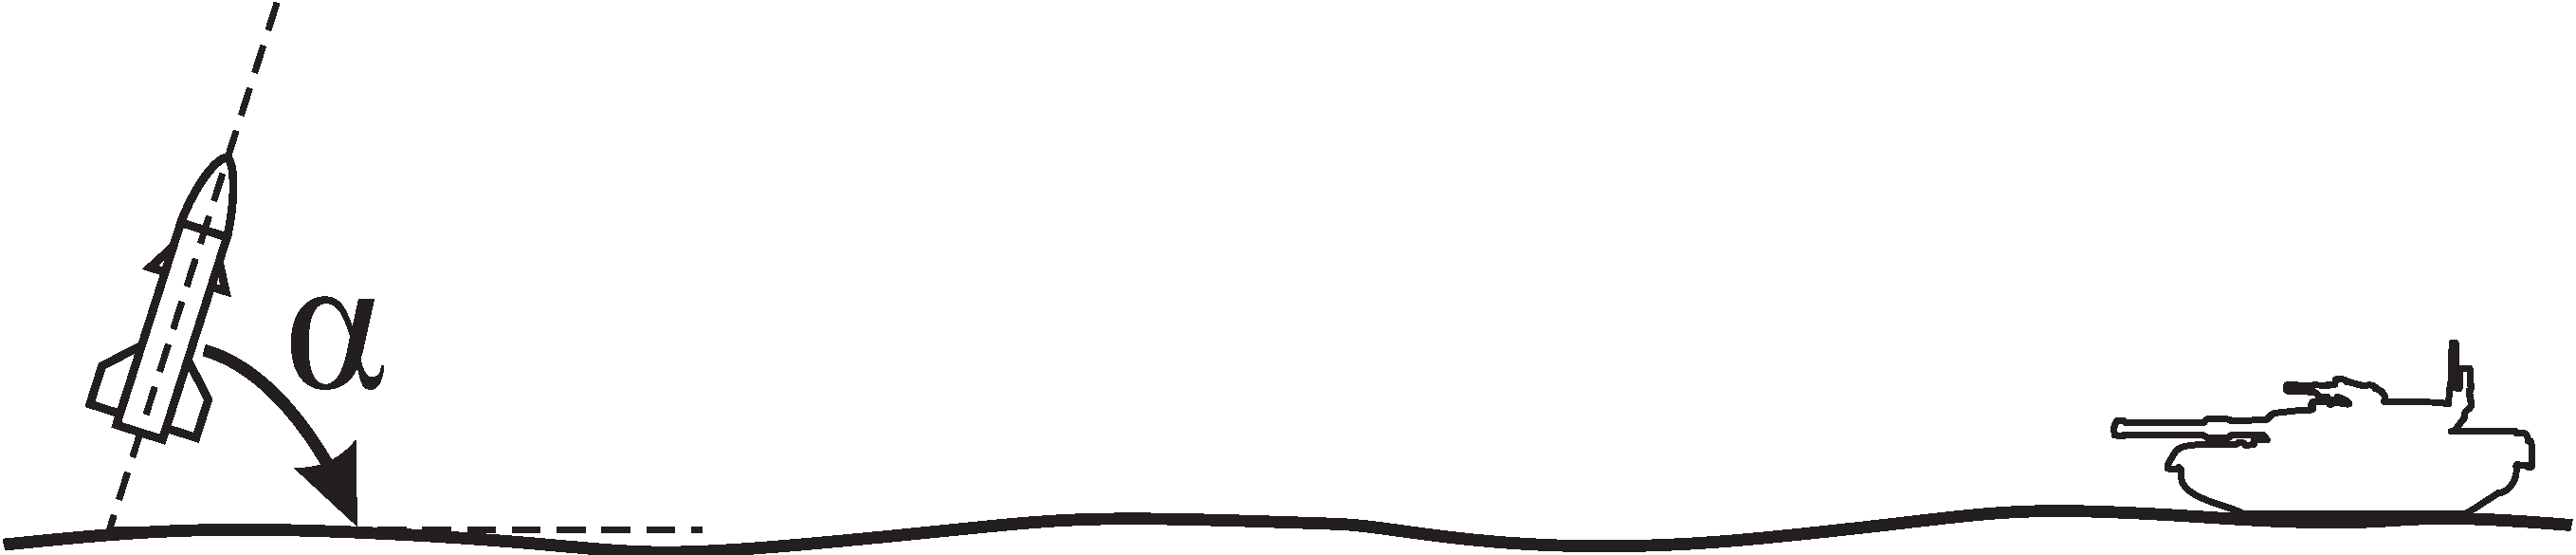
\includegraphics[width=0.475\textwidth]{rys05/alfa1} & 
  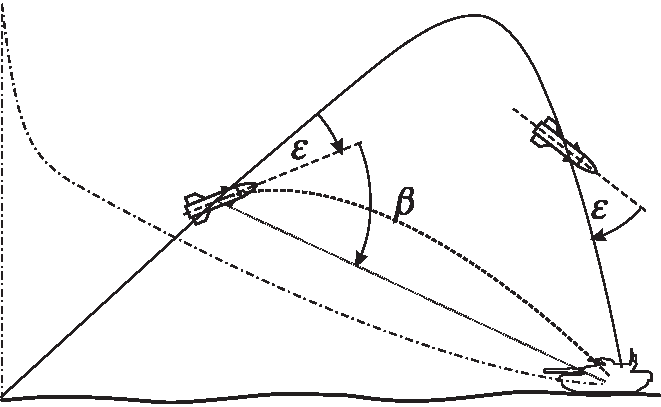
\includegraphics[width=0.475\textwidth]{rys05/beta1}
  \end{tabular}
 \caption{Wyznaczanie trajektorii lotu rakiety: 
 a) trzy podejścia, b) podejście praktyczne}
 \label{fig:alfabeta}
\end{figure}
\end{lstlisting}

\begin{figure}[ht]
	\centering
		
\includegraphics[width=0.3\linewidth]{rys05/kanji-giri}
	\caption{Dwa znaki kanji -- giri}
	\label{fig:kanji-giri}
\end{figure}

\begin{figure}[htb]
  \centering
	\begin{tabular}{@{}ll@{}}
	a) & b) \\
  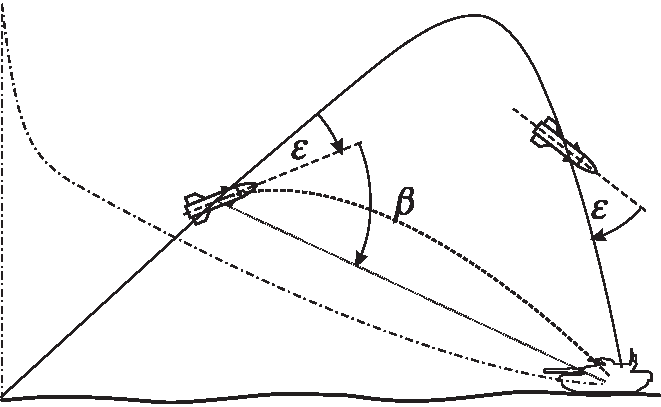
\includegraphics[width=0.475\textwidth]{rys05/beta1} & 
	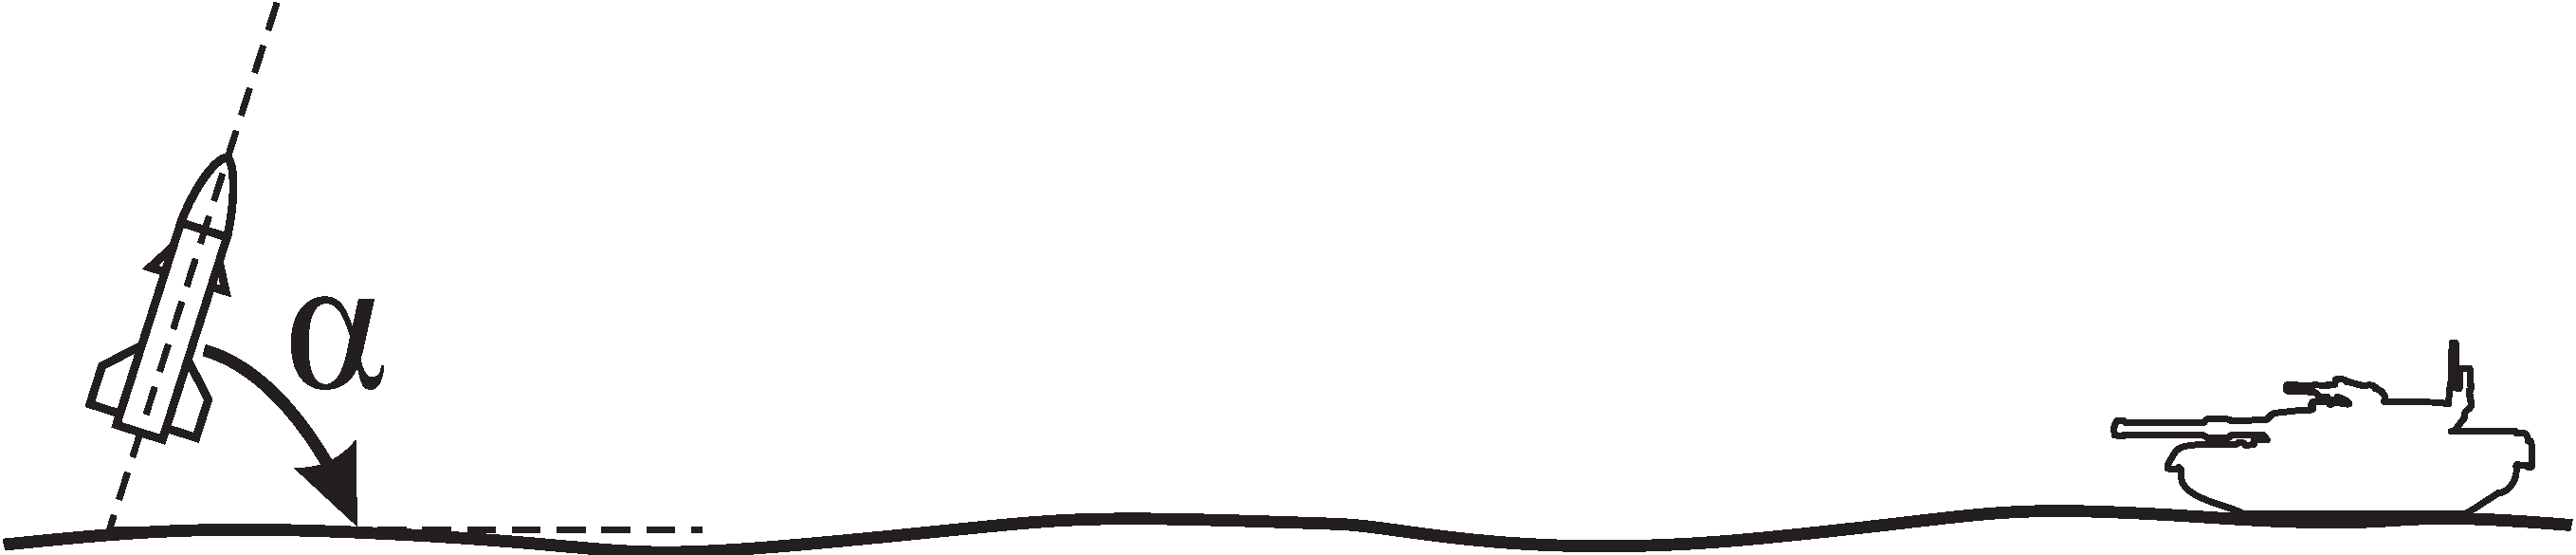
\includegraphics[width=0.475\textwidth]{rys05/alfa1}
	\end{tabular}
  \caption{Wyznaczanie trajektorii lotu rakiety: a) trzy podejścia, b) podejście praktyczne}
  \label{fig:alfabeta}
\end{figure}

Grafiki wektorowe powinny być dostarczone w plikach o formacie pdf. Rozmiar strony w~pliku pdf powinien być troszeczkę większy niż zamieszczona na nim grafika (proszę spojrzeć na przykłady grafik wykorzystanych w niniejszym szablonie). Chodzi o to, aby na rysunku nie pojawiała się niepotrzebna biała przestrzeń. Grafiki rastrowe (głównie zrzuty z ekranu bądź zdjęcia) powinny być dostarczane w plikach o formacie png z~kompresją bezstratną. Zastosowanie kompresji stratnej, jak jpg, wprowadza niepotrzebne artefakty. Podobnie jak w przypadku grafik wektorowych, grafiki rastrowe nie powinny mieć białych marginesów.

Na rysunkach nie powinno stosować się 100\% czarnego wypełnienia, bo robią się plamy przebijające się przez kartkę. Zamiast tego wypełnienie powinno być ok.\ 90\% czerni.

Czcionka na rysunkach nie może być większa od czcionki wiodącej tekstu (jedyny wyjątek to np.\ jakieś nagłówki).
Należy stosować czcionkę kroju Arial, Helvetica bądź tego samego kroju co czcionka dokumentu (\texttt{texgyre-termes}). 

Jeśli na jednym rysunku pojawić się ma kilka grafik, to zamiast stosować \texttt{subfigure} lub inne otoczenia należy wstawić grafiki w tabelę, opisać ją indeksami a) i b), a potem odnieść się do tego w podpisie (rys.~\ref{fig:alfabeta}).
Czasem pomaga w pozycjonowaniu rysunków użycie komendy:
\verb+\vtop{\vskip3ex\hbox{\includegraphics[width=0.475\textwidth]{nazwa}}}+

Na rysunkach nie wolno nadużywać kolorów oraz ozdobników (wiele narzędzi do tworzenia diagramów dostarcza grafikę z cieniowaniem, gradacją kolorów itp.\  co niekoniecznie przekłada się na czytelność rysunku).

Podczas rozbienia zrzutów z ekranu należy zadbać o to, by taki zrzut był czytelny po wydrukowaniu. Czyli aby pojawiające się literki były wystarczająco duże, a przestrzenie bez treści -- relatywnie małe.
Przystępując do robienia zrzutu trzeba odpowiednio wyskalować elementy na ekranie. Na przykład robiąc zrzut z przeglądarki FF najpierw należy wcisnąć CTR--0 (domyślne skalowanie), potem CTR--{}- (zmniejszenie skali o stopień). Potem dobrze jest zawęzić okno przeglądarki tak, by interesująca treść wypełniła je w całości. Jeśli na obserwowanej stronie jest zbyt dużo pustych obszarów, to należy je jakoś zawęzić (sterując wielkością okna przeglądarki lub aktywnymi elementami interfejsu użytkownika). Zrzut bowiem wcale nie musi być odzwierciedleniem 1:1 domyślnego układu obserwowanych elementów. Ważne jest, by na zrzucie z ekranu pokazać interesujący, opisywany fragment i żeby ten fragment był czytelny.
	
Czasem problemem jest tworzenie zrzutów z ekranu, gdy występują na nim dane wrażliwe. Istnieją dwa sposoby na radzenie sobie z tym problemem.
Pierwszy polega na zastąpieniu w~systemie danych danych rzeczywistych danymi testowymi -- wygenerowanymi tylko do celów prezentacji.
Zrzut robi się wtedy na bazie danych testowych.
Drugi polega na wykonaniu zrzutu z~ekranu, na którym pokazano dane rzeczywiste, i następnie zamianie tych danych już w pliku graficznym
za pomocą odpowiedniego edytora (np.~\texttt{gimp}). Czyli oryginalny zrzut z ekranu należy otworzyć w edytorze, a potem
nadpisać oryginalny tekst własnym tekstem. Konieczne jest wtedy dobranie odpowiednich czcionek aby nie było widać
wprowadzonych zmian. 
\begin{quotation}
Uwaga: takie manipulowanie zrzutami jest usprawiedliwione jedynie w przypadku konieczności ochrony danych wrażliwych czy też lepszego pokazania wybranych elementów. Nie może to prowadzić generowania fałszywych rezultatów!!!
\end{quotation}

\section{Wstawianie kodu źródłowego}
Kod źródłowy można wstawiać jako blok tekstu pisany czcionką maszynową. Używa się do tego otoczenie \verb?\lstlisting?. W atrybutach otoczenia można zdefiniować tekst podpisu wstawianego wraz z numerem nad blokiem, etykietę do tworzenia odwołań, sposób formatowania i~inne ustawienia. Zaleca się stosowanie w tym otoczeniu następujących parametrów:
\begin{lstlisting}[basicstyle=\footnotesize\ttfamily]
\begin{lstlisting}[label=list:req1,caption=Initial HTTP Request,
                   basicstyle=\footnotesize\ttfamily]
\end{lstlisting}
Szczególnie przydatne podczas wstawiania większej ilości kodu źródłowego jest zastosowanie parametru \verb+basicstyle=\footnotesize\ttfamily+. Dzięki niemu zmniejsza się czcionka, a~przez to na stronie można zmieścić dłuższe linijki kodu. Użycie tak zdefiniowanego parametru nie jest jednak sztywnym zaleceniem. Wielkość czcionki można dobierać do potrzeb. 
{\belowcaptionskip=-10pt
\begin{lstlisting}[label=list:req1,caption=Initial HTTP Request,
                   basicstyle=\footnotesize\ttfamily]
GET /script/Articles/Latest.aspx HTTP/1.1
Host: www.codeproject.com
Connection: keep-alive
Cache-Control: max-age=0
Accept: text/html,application/xhtml+xml,application/xml
User-Agent: Mozilla/5.0 ...
Accept-Encoding: gzip,deflate,sdch
Accept-Language: en-US...
Accept-Charset: windows-1251,utf-8...
\end{lstlisting}
}
Można też sformatować kod bez stosowania numerowanego podpisu (wtedy nie zamieszcza się \texttt{caption} na liście atrybutów).
\begin{lstlisting}[basicstyle=\footnotesize\ttfamily]
GET /script/Articles/Latest.aspx HTTP/1.1
Host: www.codeproject.com
Connection: keep-alive
Cache-Control: max-age=0
Accept: text/html,application/xhtml+xml,application/xml
User-Agent: Mozilla/5.0 ...
Accept-Encoding: gzip,deflate,sdch
Accept-Language: en-US...
Accept-Charset: windows-1251,utf-8...
\end{lstlisting}

Istnieje możliwość wstawiania kodu źródłowego w bieżącej linijce tekstu. Można to zrobić na kilka sposobów:
\begin{itemize} 
\item korzystając z polecenia \verb?\texttt? ustawiającego czcionkę maszynową, jak w przykładzie \texttt{tutaj} (efekt zastosowania komendy \verb?\texttt{tutaj}?). Problemem jednak mogą okazać się znaki podkreślenia i inne znaki kontrolne.
\item korzystają z otoczenia \verb?\verb? zapewniającego wypisanie kodu czcionką maszynową jak w~przykładzie \verb|tutaj| (efekt zastosowania komendy \verb?\verb|tutaj|?). Problemem jest to, że polecenie \verb?\verb? nie potrafi łamać dłuższego tekstu.
\item korzystając z polecenia \verb?\lstin? umożliwiającego wypisanie kodu czcionką ustawianą w~opcjach jak w przykładzie
\lstset{basicstyle=\ttfamily}\lstinline{tutaj} (efekt komendy \verb+\lstset{basicstyle=\ttfamily}\lstinline{tutaj}+) lub \lstinline[basicstyle=\ttfamily]=tutaj= (efekt komendy \verb+\lstinline[basicstyle=\ttfamily]=tutaj=+).
\end{itemize}

\section{Wykaz literatury oraz cytowania}
\label{sec:literatura}
Cytowania powinny być zamieszczane w tekście z użyciem komendy \verb+\cite{}+. Jej argumentem powinien być klucz cytowanej pozycji (lub lista kluczy  rozdzielonych przecinkiem bez spacji, jeśli takich pozycji w danym miejscu cytuje się więcej) jaki jest używany w bazie danych bibliograficznych (plik \texttt{dokumentacja.bib}). Po kompilacji \texttt{bibtex} i \texttt{pdflatex} w tekście pojawia się właściwy odsyłacz do pozycji w wykazie literatury (ujęty w kwadratowe nawiasy -- zgodnie z~tym, co definiuje styl \texttt{plabbrv.bst}), zaś w samym wykazie (rozdział Literatura) -- zacytowana pozycja. Przykładem cytowania jest: ,,dobrze to opisano w pracach~\cite{JS07,SQL2}'' (gdzie zastosowano komendę \verb?\cite{JS07,SQL2}?).

Co do zawartości rekordów bibliograficznych - style bibtexowe potrafią ,,skracać'' imiona (czyli wstawiać, jeśli taka wola, inicjały zamiast pełnych imion). Niemniej dobrze jest od razu przyjąć jakąś konwencję. Proponuje się, aby w rekordach od razu wstawiane były inicjały zamiast pełnych imion.

Niekiedy tytuły prac zawierają wyrazy z dużymi i małymi literami. Takie tytuły należy brać w podwójne nawiasy klamrowe, aby \texttt{bibtex} nie zamienił ich na postać, w której poza pierwszą literą pozostałe są małe.

Jeśli jakiś cytowany zasób pochodzi z Internetu, to jego rekord w pliku \texttt{bib} powinien wyglądać jak niżej.
\begin{lstlisting}[basicstyle=\footnotesize\ttfamily]
@INPROCEEDINGS{SQL2, 
  title={{A MySQL-based data archiver: preliminary results}}, 
  author={Bickley, M. and Slominski, Ch.},
  booktitle = {{Proceedings of ICALEPCS07}},
	month = oct,
	day = {15--19},
	year={2007}, 
  note={\url{http://www.osti.gov/scitech/servlets/purl/922267} 
	[dostęp dnia 20 czerwca 2015]}
}
\end{lstlisting}
A to inny przykład rekordu danych bibliograficznych:
\begin{lstlisting}[basicstyle=\footnotesize\ttfamily]
@TechReport{JS07,
	author = {Jędrzejczyk, J. and Śródka, B.},
	title  ={Segmentacja obrazów metodą drzew decyzyjnych},
	year = {2007},
	institution = {Politechnika Wrocławska, Wydział Elektroniki}
}
\end{lstlisting}

\section{Indeks rzeczowy}
\label{sec:indeks}
Generowanie indeksu \index{generowanie!-- indeksu} po trosze wygląda jak generowanie wykazu literatury \index{generowanie!-- wykazu literatury}-- wymaga kilku kroków. Podczas pierwszej kompilacji \texttt{pdflatex} generowany jest plik z rozszerzeniem \texttt{*.idx} (zawierający ,,surowy indeks''). Następnie, bazując na tym pliku, generowany jest plik z rozszerzeniem \texttt{*.ind} zawierający sformatowane dane. Ten krok wymaga uruchomienia odpowiedniego narzędzia oraz zastosowania plik z definicją stylu \texttt{Dyplom.ist}. W kroku ostatnim dokonuje się kolejnej kompilacji \texttt{pdflatex} (dzięki niej w wynikowym dokumencie pojawi się Indeks rzeczowy). Domyślnie Indeks rzeczowy zostanie sformatowany w~układzie dwukolumnowym.

Oczywiście aby to wszystko zadziałało w kodzie szablonu należy umieścić odpowiednie komendy definiujące elementy indeksu rzeczowego (\verb?\index?) oraz wstawiające sformatowany Indeks rzeczowy do dokumentu wynikowego (\verb?\printindex?). Więcej informacji o tworzeniu indeksu rzeczowego można znaleźć na stronie \url{https://en.wikibooks.org/wiki/LaTeX/Indexing}. Poniżej przedstawiono przykłady komend użytych w szablonie do zdefiniowania elementów indeksu rzeczowego:
\begin{itemize}
\item \verb?\index{linia komend}? -- pozycji główna.
\item \verb?\index{generowanie!-- indeksu}? -- podpozycja.
\end{itemize}

Generowanie pliku \texttt{*.ind} można inicjować na kilka sposobów:
\begin{itemize}
\item poprzez wydanie odpowiedniego polecenia bezpośrednio w linii komend \index{linia komend}
\begin{lstlisting}[basicstyle=\footnotesize\ttfamily]
makeindex Dyplom.idx -t Dyplom.ilg -o Dyplom.ind -s Dyplom.ist
\end{lstlisting}
\item poprzez odpalenie odpowiedniego narzędzia środowiska. Na przykład w \texttt{TeXnicCenter} definiuje się tzw. \texttt{output profiles}: 
\begin{lstlisting}[basicstyle=\footnotesize\ttfamily]
makeindex "%tm.idx" -t "%tm.ilg" -o "%tm.ind" -s "%tm.ist"
\end{lstlisting}
a samo generowanie pliku \texttt{*.ind} zapewni wybranie pozycji menu \texttt{Build/Makeindex}.
\item korzystając z odpowiednio sparametryzowanych pakietów i komend wewnątrz kompilowanego dokumentu (czyli od razu przy okazji jego kompilacji).
\begin{lstlisting}[basicstyle=\footnotesize\ttfamily]
\DisemulatePackage{imakeidx}
\usepackage[noautomatic]{imakeidx} 
% jeśli chcemy, by indeks by generowany automatycznie programem makeindex:
%\usepackage[makeindex]{imakeidx} 
% a tak ponoć można przekazać opcje do programu generującego indeks:
%\makeindex[options=-s podrecznik -L polish -M lang/polish/utf8] 
%\makeindex[options=-s podrecznik]
\makeindex
\end{lstlisting}

Niestety, \texttt{makeindex} jest narzędziem, które umieszcza część pozycji w grupie \texttt{Symbols}, a~nie w grupach związanych z literkami alfabetu (w związku z czym indeksowany element zaczynający się od polskiej literki trafia do grupy \texttt{Symbols}, jak np.~\verb?\index{Światło}?\index{Światło}. Jeśli chce się zamieszczać w indeksie symbole matematyczne, to dobrze jest to robić jak w następujacym przykładzie: \verb?\index{$asterisk@$\ast$}? \index{$asterisk@$\ast$} czy też \verb?\index{c@$\mathcal{C}$}?\index{c@$\mathcal{C}$}, tj.~dostarczając przy okazji klucz do sortowania.
Lepiej w tym względzie radzą sobie inne narzędzia, jak \texttt{texindy} lub \texttt{xindy} dostępne pod linuxem. Korzystając z nich uzyskuje się grupy polskich literek w indeksie rzeczowym (hasła zaczynające się od polskich literek już nie trafiają do grupy Symbols). Przykład polecenia wydanego z linii komend, w którym wykorzystano \texttt{texindy} zamieszczono poniżej (zakładamy kodowanie plików w UTF8, można dla niniejszego szablonu zmienić na cp1250):
\begin{lstlisting}[basicstyle=\footnotesize\ttfamily]
texindy -L polish -M lang/polish/utf8 Dyplom.idx
\end{lstlisting}

To polecenie wygeneruje \texttt{Dyplom.ind} o zawartości:
\begin{lstlisting}[basicstyle=\footnotesize\ttfamily]
\begin{theindex}
  \providecommand*\lettergroupDefault[1]{}
  \providecommand*\lettergroup[1]{%
      \par\textbf{#1}\par
      \nopagebreak
  }

  \lettergroup{G}
  \item generowanie
    \subitem -- indeksu, 27
    \subitem -- wykazu literatury, 27

  \indexspace

  \lettergroup{L}
  \item linia komend, 27

  \indexspace

  \lettergroup{Ś}
  \item \'Swiat\IeC {\l }o, 28

\end{theindex}
\end{lstlisting}


\end{itemize}


Aby mieć większą kontrolę automatyczne generowanie indeksu zostało w niniejszym szablonie wyłączone (indeks trzeba wygenerować samemu, wydając polecenie \texttt{makeindex} lub zalecane \texttt{texindy}).

\section{Inne uwagi}
Dobrym sposobem na kontrolę błędów występujących podczas kompilacji jest wstawiania linijki \verb?\end{document}? w wybranym miejscu dokumentu. Jest to szczególnie przydatne w przypadkach, gdy błędy te są trudne do zidentyfikowania (gdy wygenerowane przez kompilator numery linii z błędami nie są tymi, w których błędy występują). Wystarczy wtedy przestawić wspomnianą linijkę do kolejnych miejsc, aż znajduję to miejsce, gdzie występuje problem.

Aby osiągnąć apostrofy maszynowe (czyli takie złożone z samych kresek) należy użyć polecenia \verb?"{}jak tutaj{}"? (podwójny apostrof i podwójny apostrof z na wszelki wypadek umieszczonymi nawiasami klamrowymi, nawiasy są potrzebne z tej racji, iż podwójny apostrof przed niektórymi literkami zamienia je na literki z akcentami). W efekcie otrzymamy "{}jak tutaj{}". Jeśli natomiast apostrofy mają być drukarskie (czyli złożone z kropek i kresek), to należy użyć polecenia \verb?,,jak tutaj''? (dwa pojedyncze przecinki i dwa pojedyncze apostrofy). W efekcie otrzymamy ,,jak tutaj''. Można też użyć znaków apostrofów odpowiednio zakodowanych „jak tutaj”, tylko że czasem trudno pisze się takie apostrofy w środowiskach kompilacji projektów latexowych.


Oto sposoby ustawienia odstępów między liniami:
\begin{itemize}
\item używając komendy \verb+\linespread{...}+ (akceptowalne), przy czym atrybutem tej metody jest współczynnik zależny od wielkości
czcionki.  Dla czcionki wiodącej 12pt odstęp półtora linii osiągnie się komendą \verb+\linespread{1.241}+. Dla innych czcionek wiodących wartości tego parametru są jak w poniższym zestawieniu.
\begin{lstlisting}[basicstyle=\footnotesize\ttfamily]
10pt 1.25 dla \onehalfspacing 
     1.667 for \doublespacing, 
		 ponieważ ,,basic ratio'' = 1.2 
		(\normalfont posiada \baselineskip rozmiaru 12pt)
11pt 1.213 dla \onehalfspacing oraz 1.618 dla \doublespacing, 
     ponieważ ,,basic ratio'' = 1.236 
		(\normalfont posiada \baselineskip rozmiaru 13.6pt)
12pt 1.241 dla \onehalfspacing oraz 1.655 dla \doublespacing, 
     ponieważsince ''basic ratio'' is 1.208 
		(\normalfont has a \baselineskip of 14.5pt)
\end{lstlisting}
Kłopot w tym, że raz ustawiony odstęp będzie obowiązywał do wszystkich czcionek (nie działa tu żadem mechanizm zmiany współczynnika w zależności od wielkości czcionki akapitu).

\item używając pakietu \texttt{setspace} (niezalecane). Ponieważ klasa \texttt{memoir} emuluje pakiet \texttt{setspace}, w preambule dokumentu należałoby umieścić:
\begin{lstlisting}[basicstyle=\footnotesize\ttfamily]
\DisemulatePackage{setspace}
\usepackage{setspace}
\end{lstlisting}
a potem można już sterować odstęp komendami:
\begin{lstlisting}[basicstyle=\footnotesize\ttfamily]
\singlespacing
\onehalfspacing
\doubelspacing
\end{lstlisting}
Ten sposób pozwala na korzystanie z mechanizmu automatycznej zmiany odległości linii w~zależności od wielkości czcionki danego akapitu.
\item korzystając bezpośrednio z komend dostarczonych w klasie \texttt{memoir} (zalecane):
\begin{lstlisting}[basicstyle=\footnotesize\ttfamily]
\SingleSpacing
\OnehalfSpacing
\DoubleSpacing
\end{lstlisting}
Ten sposób również pozwala na korzystanie z mechanizmu automatycznej zmiany odległości linii w zależności od wielkości czcionki danego akapitu.
\end{itemize}

Na koniec jeszcze uwaga o rozmiarze pliku wynikowego. Otóż \texttt{pdflatex} generuje pliki \texttt{pdf}, które zazwyczaj mogłyby być nieco lepiej
skompresowane. Do lepszego skompresowania tych plików można użyć programu \texttt{ghostscript}. Wystarczy w tym celu wydać komendę (pod windowsami):
\begin{lstlisting}[basicstyle=\footnotesize\ttfamily]
gswin64 -sDEVICE=pdfwrite -dCompatibilityLevel=1.4 -dNOPAUSE -dQUIET -dBATCH 
-sOutputFile=Dyplom-compressed.pdf Dyplom.pdf
\end{lstlisting}

\chapter{Podsumowanie}
\label{chap:podsumowanie}
Lorem ipsum dolor sit amet eleifend et, congue arcu. Morbi tellus sit amet, massa. Vivamus est id risus. Sed sit amet, libero. Aenean ac ipsum. Mauris vel lectus. 

\section{Sekcja poziomu 1}% 
Lorem ipsum dolor sit amet eleifend et, congue arcu. Morbi tellus sit amet, massa. Vivamus est id risus. Sed sit amet, libero. Aenean ac ipsum. Mauris vel lectus. 

Nam id nulla a adipiscing tortor, dictum ut, lobortis urna. Donec non dui. Cras tempus orci ipsum, molestie quis, lacinia varius nunc, rhoncus purus, consectetuer congue risus. 

\subsection{Sekcja poziomu 2}
Lorem ipsum dolor sit amet eleifend et, congue arcu. Morbi tellus sit amet, massa. Vivamus est id risus. Sed sit amet, libero. Aenean ac ipsum. Mauris vel lectus. 
\subsubsection{Sekcja poziomu 3}
Lorem ipsum dolor sit amet eleifend et, congue arcu. Morbi tellus sit amet, massa. Vivamus est id risus. Sed sit amet, libero. Aenean ac ipsum. Mauris vel lectus. 
\paragraph{Paragraf 4}
Lorem ipsum dolor sit amet eleifend et, congue arcu. Morbi tellus sit amet, massa. Vivamus est id risus. Sed sit amet, libero. Aenean ac ipsum. Mauris vel lectus. 
\section{Sekcja poziomu 1}% 
Lorem ipsum dolor sit amet eleifend et, congue arcu. Morbi tellus sit amet, massa. Vivamus est id risus. Sed sit amet, libero. Aenean ac ipsum. Mauris vel lectus. 
%\show\chapter
%\show\section
%\show\subsection

%\showthe\secindent
%\showthe\beforesecskip
%\showthe\aftersecskip
%\showthe\secheadstyle
%\showthe\subsecindent
%\showthe\beforesubsecskip
%\showthe\aftersubsecskip
%\showthe\subseccheadstyle
%\showthe\parskip


%\bibliographystyle{plalpha}
\bibliographystyle{plabbrv}

%UWAGA: bibliotekę referencji należy przygotować samemu. Dobrym do tego narzędziem jest JabRef.
%       Nazwę przygotowanej biblioteki wpisuje się poniżej bez rozszerzenia 
%       (w tym przypadku jest to "dokumentacja.bib")
\bibliography{dokumentacja}
\appendix
\chapter{Tytuł dodatku}
Zasady przyznawania stopnia naukowego doktora i doktora habilitowanego w Polsce określa ustawa z dnia 14 marca 2003 r. o stopniach naukowych i~tytule naukowym oraz o stopniach i~tytule w zakresie sztuki (Dz.U. nr 65 z 2003 r., poz. 595 (Dz. U. z 2003 r. Nr 65, poz. 595). Poprzednie polskie uregulowania nie wymagały bezwzględnie posiadania przez kandydata tytułu zawodowego magistra lub równorzędnego (choć zasada ta zazwyczaj była przestrzegana) i zdarzały się nadzwyczajne przypadki nadawania stopnia naukowego doktora osobom bez studiów wyższych, np. słynnemu matematykowi lwowskiemu – późniejszemu profesorowi Stefanowi Banachowi. 

W innych krajach również zazwyczaj do przyznania stopnia naukowego doktora potrzebny jest dyplom ukończenia uczelni wyższej, ale nie wszędzie.


\chapter{Opis załączonej płyty CD}

W poniższych podpunktach opisano zawartość poszczególnych katalogów, które można odnaleźć na załączonej płycie CD.\\

\begin{itemize}

\item \textbf{1-dokument} - Katalog zawierający niniejszą pracę dyplomową w formacie PDF (ang. \textit{Portable Document Format}).  \\

\item \textbf{2-kod-aplikacji-serwerowej} - Katalog zawierający kompletny kod aplikacji serwerowej wraz z metadanymi systemu kontroli wersji \textit{GIT}.   \\


\item \textbf{3-skrypty-baza} - Katalog zawierający skrypty SQL służące do wdrożenia schematu bazy oraz wgrania przykładowych danych.   \\

\item \textbf{4-kod-aplikacji-klienckiej} - Katalog zawierający kompletny kod aplikacji klienckiej wraz z metadanymi systemu kontroli wersji \textit{GIT}.   \\

\item \textbf{5-zrzuty-ekranu} - Katalog zawierający zrzuty ekranu prezentujące działanie zaimplementowanego systemu.   \\

\item \textbf{6-ankiety} - Katalog zawierający ankiety wypełnione przez uczestników badań moderowanych oraz notatki moderatora.   \\

% \item \textbf{7-dokumentacja-api} - Katalog zawierający dokumentację REST API wygenerowaną za pomocą technologii \textit{Swagger}.   \\

\item \textbf{7-dostepy} - Katalog zawierający plik tekstowy z dostępami w postaci adresu wdrożonego systemu oraz danych dostępowych użytkowników testowych.

\end{itemize}





\chapterstyle{noNumbered}
\phantomsection % sets an anchor
\addcontentsline{toc}{chapter}{Indeks rzeczowy}
\printindex

\end{document}
